%=============================================================================
%  SolveBench -- Course Project Report
%  CSE 402, Numerical Analysis Lab, Department of CSE
%  Bangladesh University of Engineering and Technology
%  Compile with pdflatex (run twice for the table of contents)
%=============================================================================
\documentclass[11pt,a4paper]{article}

%------------------------------------------------ core packages
\usepackage[a4paper,top=2.4cm,bottom=2.6cm,left=2.4cm,right=2.4cm,headsep=12pt]{geometry}
\usepackage[utf8]{inputenc}
\usepackage[T1]{fontenc}
\usepackage{lmodern}
\usepackage[scaled=0.92]{helvet}
\usepackage{microtype}
\usepackage{amsmath,amssymb}
\usepackage{booktabs}
\usepackage{array}
\usepackage{longtable}
\usepackage{colortbl}
\usepackage{graphicx}
\usepackage{tikz}
\usetikzlibrary{arrows.meta,positioning,shapes.geometric,calc,fit,backgrounds,decorations.pathreplacing}
\usepackage{enumitem}
\usepackage{titlesec}
\usepackage{fancyhdr}
\usepackage{caption}
\usepackage{float}
\usepackage{tabularx}
\usepackage{multirow}
\usepackage{pifont}
\usepackage{alltt}
\usepackage[hidelinks]{hyperref}
\usepackage{bookmark}

%------------------------------------------------ palette (shared with the project's slide deck and proposal)
\definecolor{SBnavy}{RGB}{15,52,80}
\definecolor{SBteal}{RGB}{18,110,120}
\definecolor{SBgold}{RGB}{193,138,52}
\definecolor{SBgreen}{RGB}{40,120,86}
\definecolor{SBred}{RGB}{176,58,58}
\definecolor{SBbg}{RGB}{252,251,248}
\definecolor{SBgray}{RGB}{92,100,108}
\definecolor{SBlight}{RGB}{234,240,240}
\definecolor{SBlightgold}{RGB}{247,241,229}

\definecolor{HeadOne}{RGB}{86,22,125}
\definecolor{HeadTwo}{RGB}{0,102,94}
\definecolor{HeadThree}{RGB}{168,84,0}

%------------------------------------------------ section heading style
\titleformat{\section}
  {\normalfont\Large\bfseries\color{HeadOne}}
  {\thesection}{0.6em}{}
  [{\color{SBteal}\titlerule[1.1pt]}]
\titleformat{\subsection}
  {\normalfont\large\bfseries\color{HeadTwo}}
  {\thesubsection}{0.6em}{}
\titleformat{\subsubsection}
  {\normalfont\normalsize\bfseries\color{HeadThree}}
  {\thesubsubsection}{0.6em}{}
\titlespacing*{\section}{0pt}{1.6em}{0.9em}
\titlespacing*{\subsection}{0pt}{1.2em}{0.6em}
\titlespacing*{\subsubsection}{0pt}{1.0em}{0.4em}

%------------------------------------------------ header / footer
\pagestyle{fancy}
\setlength{\headheight}{12.6pt}
\fancyhf{}
\renewcommand{\headrulewidth}{0.6pt}
\renewcommand{\footrulewidth}{0.4pt}
\fancyhead[L]{\small\color{SBgray}\textit{SolveBench}}
\fancyhead[R]{\small\color{SBgray}\leftmark}
\fancyfoot[L]{\small\color{SBgray}CSE 402 Numerical Analysis Lab}
\fancyfoot[R]{\small\color{SBnavy}\thepage}
\renewcommand{\headrule}{\color{SBteal}\hrule height\headrulewidth}
\renewcommand{\sectionmark}[1]{\markboth{#1}{}}

\fancypagestyle{plain}{%
  \fancyhf{}
  \fancyfoot[L]{\small\color{SBgray}CSE 402 Numerical Analysis Lab}
  \fancyfoot[R]{\small\color{SBnavy}\thepage}
  \renewcommand{\headrulewidth}{0pt}
}

%------------------------------------------------ hyperref colours
\hypersetup{
  colorlinks=true,
  linkcolor=HeadTwo,
  citecolor=HeadTwo,
  urlcolor=HeadTwo,
  pdftitle={SolveBench -- Direct and Iterative Linear Solvers on Real Sparse Matrices},
  pdfauthor={Anuron Maitro, Md. Asif Ali, Md. Maruf Hasan Rubab, Himadri Gobinda Biswas, Md. Rafat Kabir},
  pdfsubject={CSE 402 Numerical Analysis Lab, Course Project Report},
  bookmarksopen=true,
  bookmarksdepth=3
}

%------------------------------------------------ caption style
\captionsetup{font={small,color=SBgray},labelfont={bf,color=SBnavy},labelsep=colon,margin=1cm}

%------------------------------------------------ small helper macros
\newcommand{\gd}[1]{{\color{SBgreen}\bfseries #1}}
\newcommand{\bd}[1]{{\color{SBred}\bfseries #1}}
\newcommand{\hdrow}{\rowcolor{SBnavy}}
\newcommand{\hdtxt}[1]{\textcolor{white}{\bfseries #1}}
\newcommand{\code}[1]{\texttt{\footnotesize #1}}

% shared TikZ node styles, reused directly from the project's slide deck
% (Presentation/present.tex) so every diagram in this report, the slides, and
% the proposal reads as one visual family rather than three unrelated documents
\tikzset{
  stage/.style={rounded corners=3pt,draw=SBteal,line width=1pt,fill=SBlight,
                text=SBnavy,align=center,inner sep=6pt,font=\footnotesize\bfseries,
                minimum height=1.05cm,text width=2.35cm},
  data/.style={rounded corners=3pt,draw=SBgold,line width=1pt,fill=SBlightgold,
               text=SBnavy,align=center,inner sep=6pt,font=\footnotesize,
               minimum height=1.05cm,text width=2.35cm},
  outbox/.style={rounded corners=3pt,draw=SBgreen,line width=1.2pt,fill=SBlightgold,
               text=SBnavy,align=center,inner sep=6pt,font=\footnotesize\bfseries,
               minimum height=1.05cm,text width=2.0cm},
  decision/.style={diamond,draw=SBred,line width=1pt,fill=SBred!8,
               text=SBnavy,align=center,inner sep=3pt,font=\scriptsize,
               aspect=2.2},
  milestone/.style={circle,draw=SBteal,line width=1.1pt,fill=SBlight,
               text=SBnavy,font=\scriptsize\bfseries,minimum size=0.85cm},
  fl/.style={-{Stealth[length=2.4mm]},line width=1.05pt,draw=SBteal},
  flg/.style={-{Stealth[length=2.4mm]},line width=1.05pt,draw=SBgold},
  flr/.style={-{Stealth[length=2.4mm]},line width=1.05pt,draw=SBred},
  note/.style={font=\scriptsize,text=SBgray,align=left}
}

% consistent formula panel: a thin rule above and below the formula
\newenvironment{formulabox}
  {\begin{center}\color{SBteal}\rule{0.92\linewidth}{0.8pt}\par\vspace{5pt}\color{SBnavy}}
  {\par\vspace{3pt}\color{SBteal}\rule{0.92\linewidth}{0.8pt}\end{center}}

% the same panel, set in monospace, for the pseudocode blocks in Sections 4 and 6.
% Built on alltt rather than a hand-rolled obeylines/obeyspaces regime, since alltt
% is the environment actually engineered to preserve both line breaks and leading
% indentation reliably, and function names are free to use underscores inside it.
\newenvironment{pseudobox}
  {\begin{center}\color{SBgold}\rule{0.92\linewidth}{0.8pt}\end{center}\vspace{-2pt}
   \begin{quote}\small\color{SBnavy}
   \begin{alltt}\ttfamily}
  {\end{alltt}\end{quote}\vspace{-6pt}\begin{center}\color{SBgold}\rule{0.92\linewidth}{0.8pt}\end{center}}

\renewcommand{\arraystretch}{1.15}
\newcolumntype{C}[1]{>{\centering\arraybackslash}p{#1}}

% figures live under results/figures, one level above this file
\graphicspath{{../results/figures/}}

%=============================================================================
\begin{document}
\raggedbottom

%============================================================================
% TITLE PAGE
%============================================================================
\begin{titlepage}
\pagestyle{empty}
\begin{center}

\vspace*{0.6cm}
{\large\bfseries Department of Computer Science and Engineering}\\[0.1cm]
{\large\bfseries Bangladesh University of Engineering and Technology}\\[0.1cm]
{\normalsize Dhaka, Bangladesh}

\vspace{1.0cm}
{\Huge\bfseries SolveBench}\\[0.3cm]
{\Large\bfseries Direct and Iterative Linear Solvers on Real Sparse Matrices:\\[0.15cm]
A Diagonal-Selection Pipeline for Stationary Iterative Methods}

\vspace{0.6cm}
{\color{black!40}\rule{0.65\linewidth}{0.6pt}}

\vspace{0.6cm}
{\large\bfseries Course Project Report}\\[0.2cm]
{\normalsize\bfseries CSE 402: Numerical Analysis Lab}

\vspace{0.9cm}
{\bfseries\large Submitted by}\\[0.25cm]
\begin{tabular}{p{6.8cm} c}
\toprule
\textbf{Student Name} & \textbf{Student ID} \\
\midrule
Anuron Maitro & 2105037 \\
Md.\ Asif Ali & 2105038 \\
Md.\ Maruf Hasan Rubab & 2105042 \\
Himadri Gobinda Biswas & 2105047 \\
Md.\ Rafat Kabir & 2105054 \\
\bottomrule
\end{tabular}

\vspace{0.8cm}
\begin{tabular}{ll}
\textbf{Course Teacher:} & Department of CSE, BUET \\
\end{tabular}

\vfill
{\normalsize Section A2 \quad $\cdot$ \quad Group 03}\\[0.2cm]
{\normalsize\bfseries September 2026}

\vspace*{0.2cm}
\end{center}
\end{titlepage}

\clearpage
\pagestyle{fancy}
\pagenumbering{roman}

%============================================================================
\tableofcontents
\clearpage
\listoffigures
\clearpage
\listoftables
\clearpage
\pagenumbering{arabic}
\setcounter{page}{1}

%============================================================================
\section{Introduction}
\label{sec:intro}

This report describes SolveBench, a course project built for CSE 402 that takes a small,
elegant piece of published research on Jacobi and Gauss-Seidel iteration and asks what
happens to its conclusions once real engineering matrices, rather than hand-picked or
randomly generated ones, are put in front of it. What began as a verification exercise
turned into something with more moving parts than we expected: a 927-matrix benchmark
across sixteen solver families, a discovery that over half of that corpus cannot even be
handed to the base paper's methods, and a preprocessing pipeline built in response to that
discovery, whose gains and honest costs were measured on the full corpus rather than
assumed from a smaller probe. This introduction lays out the problem, the scope of what we
built, and how the rest of the report is organized.

\subsection{The problem: solving \texorpdfstring{$A\vec{x}=\vec{b}$}{Ax=b} at scale}
\label{sec:intro-problem}

Almost every simulation of a physical system, a power grid under load, a bridge under
stress, an integrated circuit under bias, a chemical plant at steady state, eventually
reduces to one piece of linear algebra:

\begin{formulabox}
$$A\vec{x} = \vec{b}$$
\end{formulabox}

Here $A$ encodes how the parts of the system interact with each other, $\vec{b}$ is
whatever is being pushed into the system, and $\vec{x}$ is the quantity being solved for.
For a problem of any realistic size, $A$ has thousands, sometimes millions, of rows and
columns, but it is almost always \emph{sparse}: the overwhelming majority of its entries
are exactly zero, because most components of a physical system only interact with their
immediate neighbours. A resistor in a circuit is wired to the two or three nodes touching
it, not to every other node in the network.

Two broad families of technique exist for solving such a system. \textbf{Direct methods}
factor $A$ into triangular pieces, in the same spirit as Gaussian elimination done by
hand, and then solve two easy triangular systems. This produces the exact answer, up to
floating-point rounding, in a fixed and predictable number of steps, but the factorization
step can introduce a great many new nonzero entries where $A$ had zeros (\emph{fill-in}),
and for a sufficiently large sparse matrix this can exceed the memory available.
\textbf{Iterative methods} instead start from a guess, usually $\vec{x}_0 = \vec{0}$, and
repeatedly refine it, checking the residual $\|A\vec{x}-\vec{b}\|$ at every step and
stopping once it is small enough. Each step is comparatively cheap, essentially one
matrix-vector product, so iterative methods scale to far larger problems than direct
factorization can reach. The catch is that nothing guarantees the steps actually approach
the answer; whether they do depends entirely on the structure of $A$, and that dependency
is the subject of this entire project.

\subsection{Problem statement}
\label{sec:intro-statement}

The concrete question this project set out to answer is simple to state and, as it
turned out, considerably harder to answer honestly than we expected at the outset:

\begin{itemize}[leftmargin=1.4cm]
  \item A well-known paper (Section~\ref{sec:motivation-paper}) derives, by hand, exactly
  which small matrices make Jacobi and Gauss-Seidel converge, and validates that theory
  statistically on randomly generated matrices with at most five unknowns. \textbf{Does
  any of that survive contact with the matrices that working engineers actually have to
  solve, at the sizes those matrices actually come in?}
  \item Where the classical iterative methods do fail, is the failure a property of the
  \emph{matrix}, in which case nothing can be done about it short of switching solver
  families, or is it a property of an arbitrary, fixable choice made somewhere upstream of
  the solver, such as the order in which the matrix's rows happen to be listed?
  \item If some of that failure is fixable, how much of it, by what mechanism, and at what
  cost? A preprocessing step that helps on paper but costs more than it saves, or that
  quietly breaks some other case while fixing this one, is not a contribution; it is a
  trade that needs to be measured, not assumed.
\end{itemize}

\subsection{Scope and objectives}
\label{sec:intro-scope}

As actually built and measured, the project delivers the following, each of which is
described in full later in this report:

\begin{itemize}[leftmargin=1.4cm]
  \item A from-scratch implementation of Jacobi, Gauss-Seidel, and Successive
  Over-Relaxation (SOR), together with the classical convergence theory that governs them,
  built independently of any existing solver library (Section~\ref{sec:methods}).
  \item A benchmark harness that runs sixteen solver methods, spanning direct, stationary
  iterative, Krylov, and preconditioned families, across every matrix in a
  927-matrix corpus drawn from the SuiteSparse Matrix Collection, with success decided
  independently from the measured residual rather than from any solver's own claim
  (Section~\ref{sec:datasets}, Section~\ref{sec:results}).
  \item A diagnosis of why the classical stationary methods are unusable on more than half
  of that corpus before a single iteration is attempted, and a proof, not merely a guess,
  of which preprocessing operations could possibly change that (Section~\ref{sec:novel}).
  \item A preprocessing pipeline, built on that proof, that chooses which row of the
  matrix sits on the diagonal and, for SOR, chooses its relaxation factor per matrix, and
  a full measurement of what that pipeline does and does not buy
  (Section~\ref{sec:novel}, Section~\ref{sec:results}).
  \item A dedicated failure analysis, carried out once every arm of the pipeline had
  finished running, that explains precisely why the classical methods fail and why the
  project's own bottleneck objective, though it wins decisively on the quantity it was
  built to minimise, converts only a modest number of additional systems
  (Section~\ref{sec:failure}).
\end{itemize}

The project deliberately targets square, real-valued sparse matrices with at most ten
thousand rows and columns; it does not attempt multigrid or domain-decomposition methods,
GPU or distributed execution, or wall-clock performance engineering, and it does not
propose a new iterative method. Every one of these boundaries is a considered decision,
not an oversight, and each is revisited where it matters in the discussion
(Section~\ref{sec:discussion}).

\subsection{How this report is organized}
\label{sec:intro-organization}

Section~\ref{sec:motivation} introduces the base paper this project extends and places it
against the small body of related work on diagonal reordering for iterative solvers.
Section~\ref{sec:datasets} describes the SuiteSparse-derived corpus in detail, with
concrete named examples. Section~\ref{sec:methods} covers every method implemented
directly from the base paper, together with the classical convergence theory and the
additional solver families built so the comparison would have a floor and a ceiling.
Section~\ref{sec:novel} tells the story of the project's own contribution as it actually
happened, milestone by milestone, including the false starts. Section~\ref{sec:results}
reports every measured number behind the headline claims. Section~\ref{sec:failure} is a
dedicated failure analysis, requested specifically for this report, that explains why each
solver family fails on this corpus and how both the classical methods and our own designed
methods were investigated and, where possible, improved in response. Section~\ref{sec:discussion}
discusses honest strengths and limitations and points to future work, and
Section~\ref{sec:conclusion} closes the report.

\clearpage
%============================================================================
\section{Motivation and Related Work}
\label{sec:motivation}

\subsection{The base paper: Khrapov and Volkov, 2024}
\label{sec:motivation-paper}

This project extends a specific, published piece of research: P. Khrapov and N. Volkov,
\emph{Comparative Analysis of Jacobi and Gauss-Seidel Iterative Methods}, International
Journal of Open Information Technologies, vol. 12, no. 2, pp. 23--34, 2024. The paper
studies the two oldest and simplest stationary iterative methods for $A\vec{x}=\vec{b}$.
For systems of two and three unknowns, the authors derive, algebraically and by hand, the
precise region of coefficient space in which each method converges and in which it
diverges. They then generate a large number of random matrices with up to five unknowns
and check, empirically, how often the derived theory holds.

What the paper does not do is, in a sense, more informative than what it does. It never
once evaluates a matrix that came from an actual engineering problem. Every matrix
studied is either small enough to be solved by hand or generated by a random-number
routine, and a randomly generated matrix does not resemble a real one in any structural
sense. A matrix that comes from a circuit simulator, a finite-element mesh, or a
power-flow model carries a specific, non-random pattern of zero and nonzero entries
determined by which physical components are actually connected to which others. This is
precisely the gap this project set out to close: nobody, as far as we could determine, had
checked whether the base paper's conclusions survive contact with matrices that engineers
actually have to solve, at the sizes those matrices actually arrive in.

\subsection{Related work on diagonal selection for iterative solvers}
\label{sec:motivation-related}

The idea of choosing which entry of a sparse matrix sits on the diagonal, rather than
accepting whatever order the matrix arrived in, is not new; it is a well established tool
in the numerical linear algebra literature, though almost entirely in service of a
different goal than the one this project pursues.

Duff and Koster's algorithm for permuting large entries onto the diagonal, published as
\emph{The design and use of algorithms for permuting large entries to the diagonal of
sparse matrices} (SIAM Journal on Matrix Analysis and Applications, vol. 20, pp. 889--901,
1999) and distributed widely as the routine MC64, is the standard tool this project
measures its own idea against throughout. MC64 chooses the diagonal that maximizes the
product of the diagonal magnitudes, a criterion built specifically to make subsequent
direct factorization numerically stable. Hook, Pestana, Tisseur, and Hogg extended this
line of work in \emph{Max-Balanced Hungarian Scalings} (SIAM Journal on Matrix Analysis
and Applications, vol. 40, no. 1, pp. 320--346, 2019), addressing the fact that a
maximum-product assignment is often not unique and proposing a principled way to choose
among the ties from the point of view of diagonal dominance, a concern that turns out to
be close in spirit, though not in method, to the objective this project builds in
Section~\ref{sec:novel-objective}. Benzi, Haws, and Tuma, in \emph{Preconditioning highly
indefinite and nonsymmetric matrices} (SIAM Journal on Scientific Computing, vol. 22, pp.
1333--1353, 2000), studied permutation and scaling strategies aimed specifically at
making incomplete factorizations more reliable on hard, indefinite systems, a concern that
resurfaces directly in this project's own encounter with incomplete LU preconditioning
(Section~\ref{sec:failure-ilu}). None of this prior work, to our knowledge, poses the
question this project asks: can a row permutation be chosen specifically to make the
classical stationary methods, Jacobi, Gauss-Seidel, and SOR, converge, rather than to
stabilize a direct factorization or a preconditioner. That distinction, and everything it
implies once measured honestly, is the actual substance of Section~\ref{sec:novel}.

Barrett et al.'s \emph{Templates for the Solution of Linear Systems} (SIAM, 1994) is the
standard reference for the broader family of Krylov and preconditioned methods
implemented in this project purely as context, described in
Section~\ref{sec:methods-baselines}, and it is also, as it happens, the source of a
lesson the group learned the hard way about its own original proposal, told in full in
Section~\ref{sec:novel-apk}.

\clearpage
%============================================================================
\section{Datasets}
\label{sec:datasets}

\subsection{The SuiteSparse Matrix Collection}
\label{sec:datasets-suitesparse}

The SuiteSparse Matrix Collection (Davis and Hu, \emph{The University of Florida Sparse
Matrix Collection}, ACM Transactions on Mathematical Software, vol. 38, no. 1, 2011) is
the standard public library of real, sparse matrices contributed by engineers and
scientists from actual projects, each tagged with metadata describing its size, its
number of nonzero entries, and the real-world domain it came from. This is what lets the
project ask a question the base paper's random matrices cannot: does Gauss-Seidel
actually work on a circuit-simulation matrix, rather than does it work on numbers chosen
uniformly at random.

\subsection{Selection rule and corpus bookkeeping}
\label{sec:datasets-bookkeeping}

The selection rule is every square, real-valued matrix in the collection with at most ten
thousand rows and columns. That cap is a memory limit, not a judgement about difficulty:
one of the project's analyses computes the exact spectral radius of the iteration matrix,
which requires a dense $n \times n$ array, and at $n = 10{,}000$ that array alone already
occupies roughly 800 megabytes. The collection holds 1{,}184 matrices meeting this size
criterion; this project draws a sample of 830 of them, not a complete census, together
with 100 matrices generated by the project itself specifically to reproduce the base
paper's own validation approach at larger scale, for a nominal total of 930 downloaded
files.

That nominal total needs three corrections before any result can be trusted. Three files
are exact byte-for-byte duplicates of other files under a different name
(\code{bcsstk07}$\equiv$\code{bcsstk06}, \code{bcsstk12}$\equiv$\code{bcsstk11},
\code{t2dal\_a}$\equiv$\code{t2dal}), bringing the unique corpus to \textbf{927 matrices}.
Six further files turned out to be truncated downloads, each one's own header declaring
more nonzero entries than the file physically contained, so they fail to load at all
(\code{cavity20}, \code{nemeth17}, \code{nemeth22}, \code{nemeth23}, \code{nemeth25},
\code{psmigr\_2}); Section~\ref{sec:failure-mistakes} explains how this was caught. Finally,
one physical domain, computational fluid dynamics, arrived split across two folders
because SuiteSparse's own metadata spells it two different ways depending on which
research group contributed the matrix; the two are merged for every table and figure in
this report. None of these corrections change any conclusion reported later; they only
change which denominator a rate is computed against, and every table in this report states
that denominator explicitly rather than leaving it implicit.

\subsection{The 26 domains}
\label{sec:datasets-domains}

Table~\ref{tab:domains} lists every domain in the corpus with its matrix count. The
distribution is sharply uneven: one domain alone, circuit simulation, contributes over a
fifth of the entire corpus, while eight domains contribute fewer than five matrices each.
This is not a defect in the corpus; it is a fact about which of these problems
practitioners happen to solve most often, and it is the reason every per-domain claim
made anywhere in this report states its own denominator rather than leaving the reader to
assume a comparable sample size across domains.

\begin{table}[H]
\centering
\caption{The 26 real-world domains represented in the corpus, by matrix count.}
\label{tab:domains}
\small
\begin{tabular}{lr}
\toprule
\hdrow \hdtxt{Domain} & \hdtxt{Matrices} \\
\midrule
Circuit simulation & 200 \\
\rowcolor{SBlight} Computational fluid dynamics & 121 \\
Random matrices (self-generated) & 100 \\
\rowcolor{SBlight} Structural engineering & 87 \\
Optimal control & 78 \\
\rowcolor{SBlight} 2D/3D discretization & 49 \\
Chemical process simulation & 44 \\
\rowcolor{SBlight} Optimization & 39 \\
Undirected weighted graph & 37 \\
\rowcolor{SBlight} Theoretical quantum chemistry & 27 \\
Electromagnetics & 25 \\
\rowcolor{SBlight} Eigenvalue / model reduction & 19 \\
Directed weighted graph & 17 \\
\rowcolor{SBlight} Power network & 17 \\
Economic modelling & 16 \\
\rowcolor{SBlight} Model reduction & 13 \\
Materials & 9 \\
\rowcolor{SBlight} Statistical / mathematical & 6 \\
Counter-example & 4 \\
\rowcolor{SBlight} Semiconductor device & 4 \\
Acoustics & 2 \\
\rowcolor{SBlight} Thermal & 2 \\
Computational chemistry & 1 \\
\rowcolor{SBlight} Computer graphics / vision & 1 \\
Linear programming & 1 \\
\rowcolor{SBlight} Robotics & 1 \\
\bottomrule
\end{tabular}
\end{table}

\begin{figure}[H]
\centering
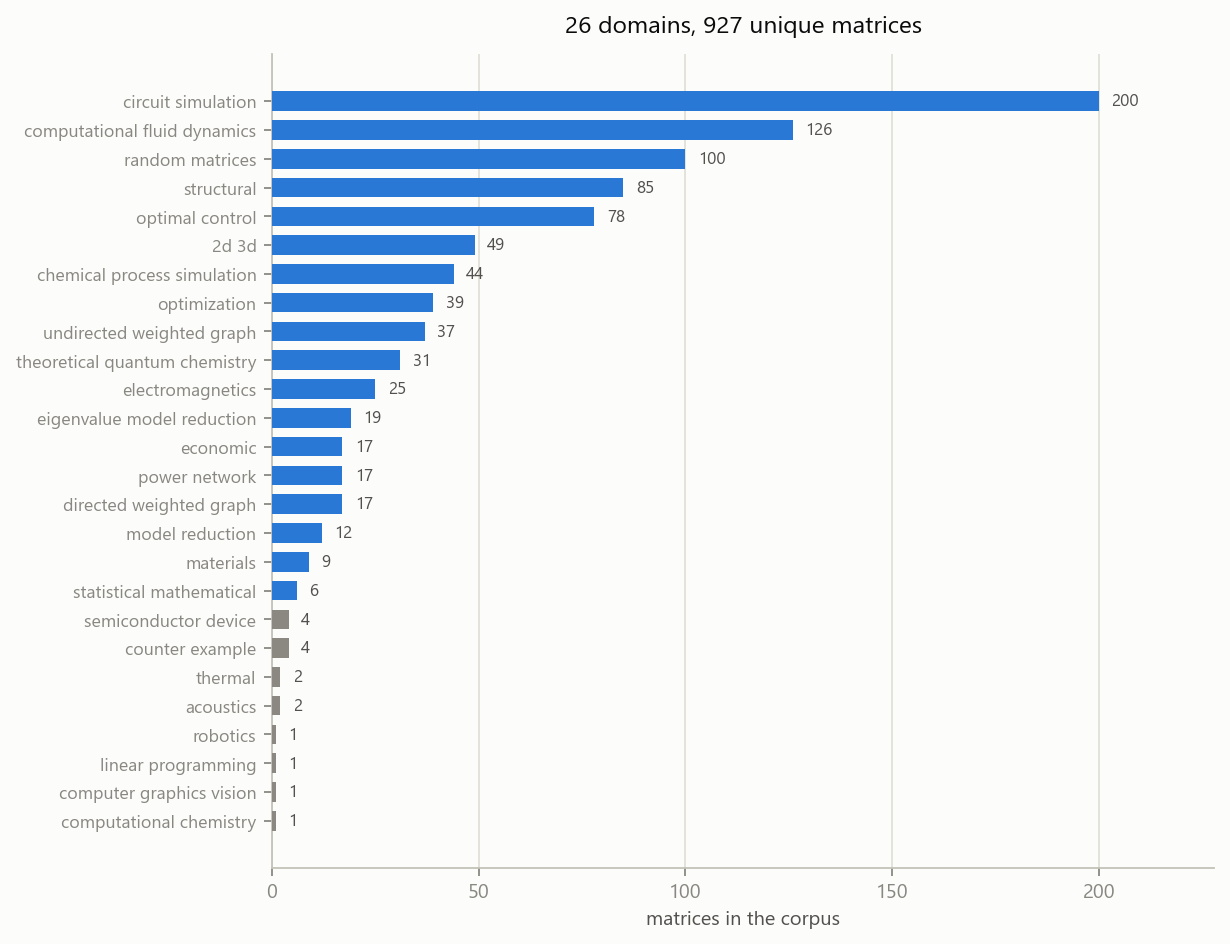
\includegraphics[width=0.82\linewidth]{22_domain_composition.png}
\caption{Domain composition of the 927-matrix corpus, drawn to scale. Circuit simulation
and computational fluid dynamics together account for close to a third of the entire
corpus, while more than half of the 26 domains have fewer than 25 matrices apiece.}
\label{fig:domain-composition}
\end{figure}

\subsection{Concrete examples}
\label{sec:datasets-examples}

Table~\ref{tab:examples} names specific matrices from the corpus so that later claims in
this report can be traced back to an actual, inspectable system rather than staying
abstract.

\begin{table}[H]
\centering
\caption{Representative matrices from the corpus, by domain, size, and nonzero count.}
\label{tab:examples}
\small
\begin{tabular}{llrr}
\toprule
\hdrow \hdtxt{Domain} & \hdtxt{Matrix} & \hdtxt{Size ($n$)} & \hdtxt{Nonzeros} \\
\midrule
Circuit simulation & \code{meg1} & 2,904 & 58,142 \\
\rowcolor{SBlight} Circuit simulation & \code{circuit\_1} & 2,624 & 35,823 \\
Structural engineering & \code{Kuu} & 7,102 & 173,651 \\
\rowcolor{SBlight} Structural engineering & \code{raefsky5} & 6,316 & 168,658 \\
Fluid dynamics & \code{ex40} & 7,740 & 458,012 \\
\rowcolor{SBlight} Fluid dynamics & \code{GT01R} & 7,980 & 430,909 \\
Power network & \code{TSC\_OPF\_1047} & 8,140 & 1,012,521 \\
\rowcolor{SBlight} Power network & \code{TSC\_OPF\_300} & 9,774 & 415,289 \\
Quantum chemistry & \code{nemeth26} & 9,506 & 760,633 \\
\rowcolor{SBlight} Economic modelling & \code{psmigr\_3} & 3,140 & 543,162 \\
Electromagnetics & \code{fp} & 7,548 & 848,553 \\
\rowcolor{SBlight} Self-generated random & \code{rand\_100\_n300} & 300 & 90,000 \\
\bottomrule
\end{tabular}
\end{table}

\begin{figure}[H]
\centering
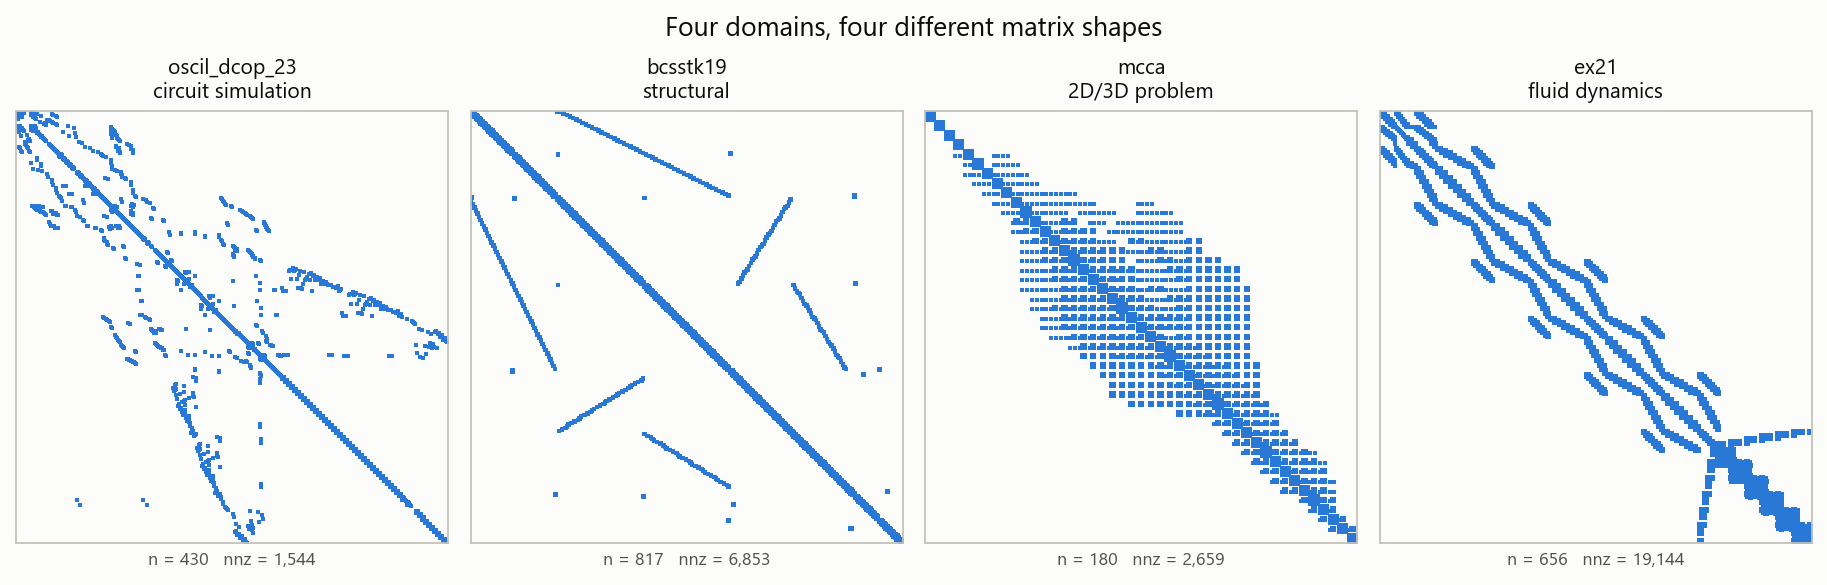
\includegraphics[width=0.9\linewidth]{18_matrix_gallery.png}
\caption{Sparsity patterns of a gallery of corpus matrices spanning several domains. Each
panel is the same square canvas at the same visual scale; the density and banding
differences between, say, a circuit-simulation matrix and a structural one are a direct,
visible reason the two behave so differently under an iterative solver.}
\label{fig:matrix-gallery}
\end{figure}

A handful of matrices recur throughout this report by name because each one is the
concrete evidence behind a specific claim, not an anecdote. \code{cdde6} (fluid dynamics,
$n=961$) has a Jacobi spectral radius of 0.717, comfortably inside the convergent region,
yet its residual grows to 44{,}764 times its starting value before it finally shrinks and
converges at iteration 178; this single matrix is the reason the harness's divergence
guard has to be lenient, a point returned to in Section~\ref{sec:novel-harness}.
\code{d\_ss} (chemical process simulation, $n=53$) is the one matrix in the whole corpus
on which the project's own reordering objective makes the spectral radius worse, from
1.884 to 29.605, discussed honestly in Section~\ref{sec:failure-negatives}. \code{nnc261},
\code{west0067}, \code{bcsstk19}, and \code{rw5151}, four matrices from four different
domains, each separately exposed a hang in an off-the-shelf scipy matching routine, the
subject of Section~\ref{sec:novel-hangs}. \code{iprob} (linear programming, $n=3{,}001$)
is one of only four matrices in the entire corpus that the project's own bottleneck
objective rescues and the established MC64 objective does not, discussed in
Section~\ref{sec:novel-reordering-result}.

\clearpage
%============================================================================
\section{Methods Implemented From the Base Paper}
\label{sec:methods}

Every method the base paper studies was implemented independently, from first
principles, before any comparison against real data was attempted. This section presents
each one together with the convergence theory that governs it, and then describes the
further solver families added purely so the comparison would have context: a
specialised method looking good or bad in isolation means little without a floor and a
ceiling to measure it against.

\subsection{Splitting the matrix}
\label{sec:methods-splitting}

Jacobi, Gauss-Seidel, and SOR all begin from the same decomposition of the coefficient
matrix into three pieces:

\begin{formulabox}
$$A = D + L + U$$
\end{formulabox}

where $D$ holds only the diagonal entries, $L$ is everything strictly below the diagonal,
and $U$ is everything strictly above it. Every one of the three methods needs to divide by
the entries of $D$ at some point in its update rule, a fact whose consequences turn out to
be far larger than a technical footnote, as Section~\ref{sec:novel-491} describes.

\subsection{Jacobi's method}
\label{sec:methods-jacobi}

Jacobi's update uses only values from the previous complete iteration; nothing computed
so far in the current pass feeds back into itself.

\begin{pseudobox}
function JACOBI(A, b, tolerance, max_iterations):
    x <- zeros(n)
    for k in 1 .. max_iterations:
        r <- b - A @ x
        if norm(r) / norm(b) <= tolerance:
            return x, converged = true
        x <- x + r / diagonal(A)
    return x, converged = false
\end{pseudobox}

\subsection{Gauss-Seidel}
\label{sec:methods-gs}

Gauss-Seidel is the same idea with one change: each row's update can immediately use the
already-updated values from earlier rows in the same pass. This usually converges
noticeably faster than Jacobi on the same matrix, though not always, as
Section~\ref{sec:results-basepaper} measures directly.

\begin{pseudobox}
function GAUSS_SEIDEL(A, b, tolerance, max_iterations):
    x <- zeros(n)
    for k in 1 .. max_iterations:
        r <- b - A @ x
        if norm(r) / norm(b) <= tolerance:
            return x, converged = true
        solve (D + L) @ delta = r   for delta
        x <- x + delta
    return x, converged = false
\end{pseudobox}

\subsection{Successive Over-Relaxation (SOR)}
\label{sec:methods-sor}

SOR scales the Gauss-Seidel update by a relaxation factor $\omega$ before applying it,
deliberately overshooting the correction, which can converge faster than plain
Gauss-Seidel when $\omega$ is chosen well. Setting $\omega=1$ reduces exactly to
Gauss-Seidel.

\begin{pseudobox}
function SOR(A, b, omega, tolerance, max_iterations):
    x <- zeros(n)
    for k in 1 .. max_iterations:
        r <- b - A @ x
        if norm(r) / norm(b) <= tolerance:
            return x, converged = true
        solve (D + omega * L) @ delta = omega * r   for delta
        x <- x + delta
    return x, converged = false
\end{pseudobox}

SOR was not itself the subject of the base paper, but it is Gauss-Seidel with a single
extra tuning parameter, and that parameter turns out to matter a great deal to this
project's own contribution, described starting in Section~\ref{sec:novel-omega}.

\subsection{Convergence theory: the spectral radius}
\label{sec:methods-spectral}

Whether any of the three methods above converges at all is governed by a single number:
the spectral radius $\rho(T)$ of that method's iteration matrix $T$ (a different $T$ for
Jacobi, $T_J = -D^{-1}(L+U)$, than for Gauss-Seidel, $T_{GS}=-(D+L)^{-1}U$).

\begin{formulabox}
If $\rho(T) < 1$: the error shrinks a little further every step, eventually to zero.\\
If $\rho(T) \geq 1$: the error does not shrink; the method will not converge.
\end{formulabox}

The spectral radius also governs speed, not merely whether convergence happens at all:
reaching a tolerance $\varepsilon$ takes roughly $\log(\varepsilon)/\log(\rho(T))$ steps. A
$\rho$ of 0.5 needs about 27 steps to reach $10^{-8}$; a $\rho$ of 0.999 needs roughly
18{,}000, and, as Section~\ref{sec:failure-theorem-wall} shows, this gap between
``converges'' and ``converges usefully'' turns out to be the single most important fact
about this entire corpus.

\begin{figure}[H]
\centering
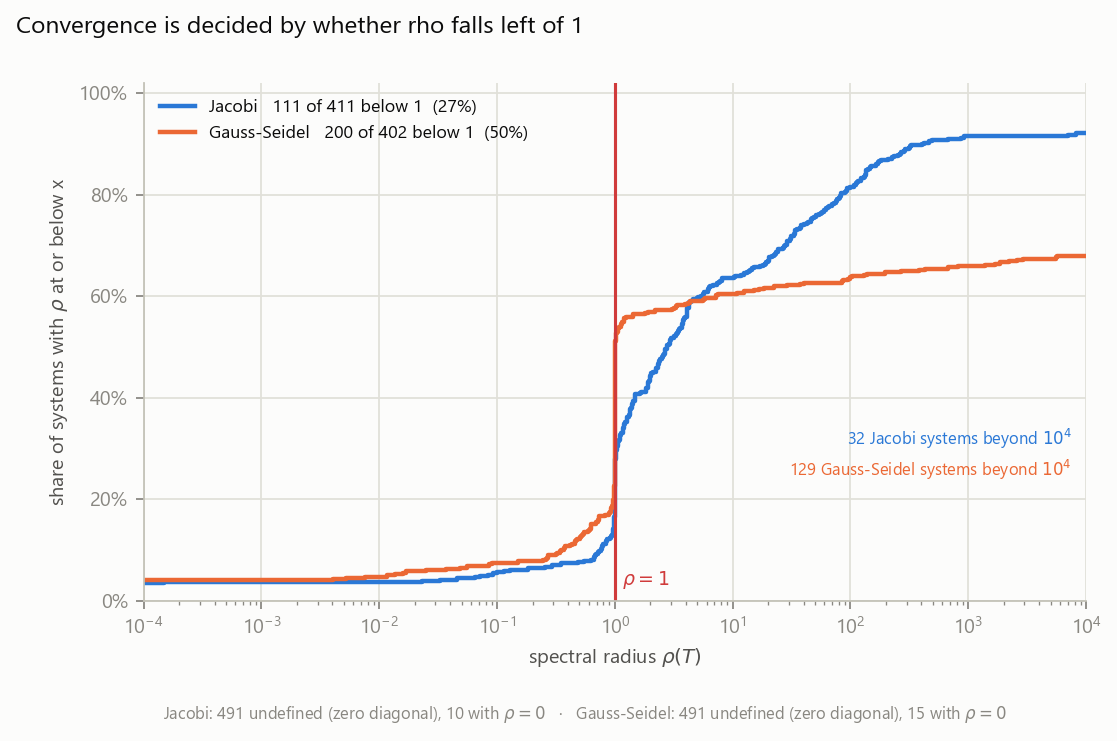
\includegraphics[width=0.82\linewidth]{11_spectral_radius.png}
\caption{Distribution of $\rho(T_{Jacobi})$ and $\rho(T_{Gauss\text{-}Seidel})$ across the
corpus. The mass sitting just above and just below 1 is not a rounding artefact; it is the
regime that decides most of what Section~\ref{sec:failure} has to explain.}
\label{fig:spectral-radius}
\end{figure}

Beyond the spectral radius itself, a family of classical sufficient conditions, strict and
weak diagonal dominance, the H-matrix, M-matrix, and L-matrix properties, symmetric
positive definiteness, and the property-A structure behind the classical
Householder-John theorem, each guarantee convergence without requiring $\rho(T)$ to be
computed directly. Figure~\ref{fig:hypothesis-coverage} shows how much of the corpus each
classical hypothesis actually covers; Section~\ref{sec:failure-theorem-wall} shows what
happens to the matrices none of them cover.

\begin{figure}[H]
\centering
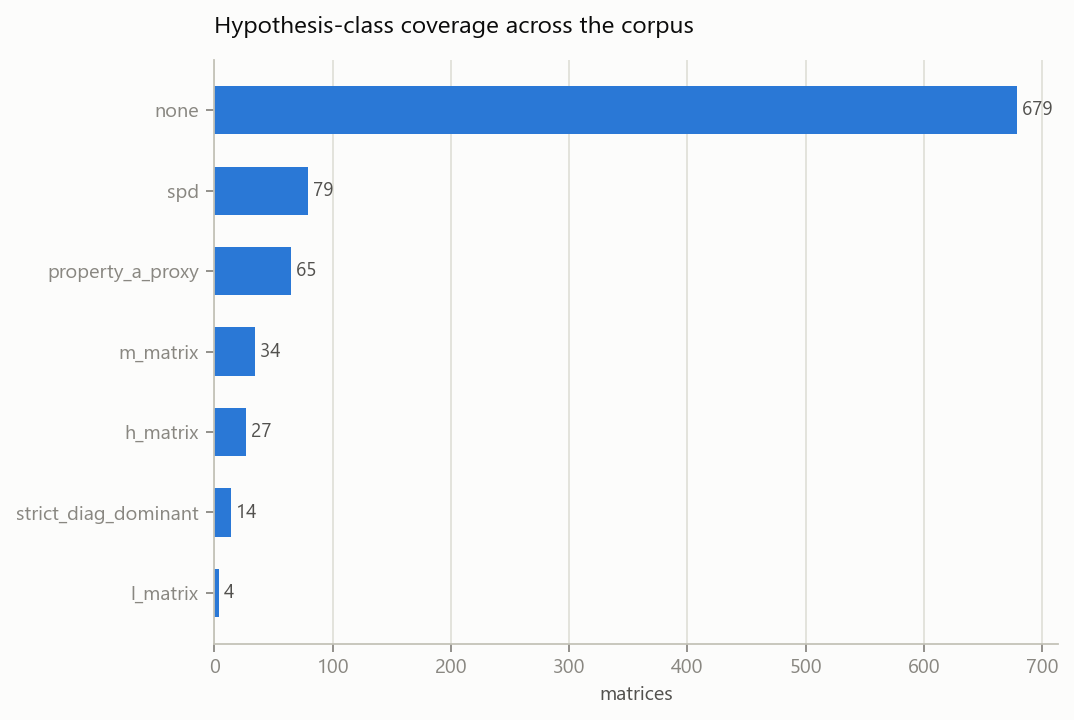
\includegraphics[width=0.82\linewidth]{12_hypothesis_coverage.png}
\caption{How many corpus matrices fall under each classical convergence-guarantee
hypothesis. The classes overlap (a strictly diagonally dominant matrix is also an
H-matrix, for instance), and a large fraction of the corpus falls under none of them.}
\label{fig:hypothesis-coverage}
\end{figure}

\subsection{Reproducing the base paper's own experiment}
\label{sec:methods-random}

To compare against the base paper on its own terms, not only on new terms of our
choosing, the project generated its own \code{random\_matrices} domain, 100 matrices
sized from 5 to 300 unknowns, following the same generation procedure as the base paper's
own validation experiment. This is a deliberate methodological choice: it lets
Section~\ref{sec:results-basepaper} report how the base paper's own test bed behaves once
matrices larger than five unknowns are allowed, rather than only reporting how our new,
larger corpus behaves, which would leave the comparison one step removed from the paper it
is meant to be checking.

\begin{figure}[H]
\centering
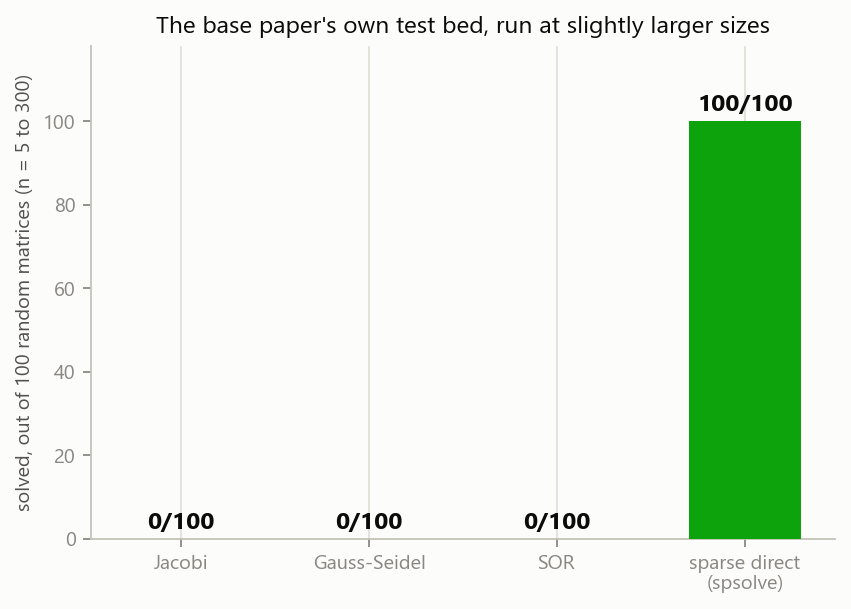
\includegraphics[width=0.82\linewidth]{23_random_matrices.png}
\caption{Spectral radius against matrix size for the self-generated random-matrix domain.
The growth is visible almost immediately past the base paper's own tested range of two to
five unknowns.}
\label{fig:random-matrices}
\end{figure}

\subsection{Additional baseline families}
\label{sec:methods-baselines}

The base paper studies exactly two methods. Reporting that Jacobi or Gauss-Seidel
succeeds or fails on some fraction of a corpus means little without something to compare
that fraction against, so thirteen further methods across three additional families were
implemented, giving sixteen methods in total.

\subsubsection{Direct methods}
\label{sec:methods-direct}

Gauss elimination, Gauss-Jordan elimination, LU decomposition, and Cholesky decomposition
were implemented by hand, in addition to the industrial-strength sparse routines
\code{spsolve} and \code{splu} from the SuperLU library accessed through scipy. Direct
methods factor the matrix once and then solve two triangular systems, giving the exact
answer, up to floating-point rounding, in a fixed number of steps, at the cost of
potentially large memory use from fill-in.

\subsubsection{Krylov methods}
\label{sec:methods-krylov}

Conjugate Gradient, BiCGSTAB, and GMRES(30) build up a small search space by repeatedly
multiplying the matrix against a vector, $\vec{b}, A\vec{b}, A^2\vec{b}, \ldots$, and pick
the best possible answer inside that space at every step, rather than following a fixed
formula the way the stationary methods do.

\begin{pseudobox}
function CONJUGATE_GRADIENT(A, b, tolerance, max_iterations):
    x <- zeros(n)
    r <- b - A @ x
    p <- r
    for k in 1 .. max_iterations:
        if norm(r) / norm(b) <= tolerance:
            return x, converged = true
        alpha <- (r . r) / (p . (A @ p))
        x <- x + alpha * p
        r_new <- r - alpha * (A @ p)
        beta <- (r_new . r_new) / (r . r)
        p <- r_new + beta * p
        r <- r_new
    return x, converged = false
\end{pseudobox}

Conjugate Gradient is valid only on symmetric positive-definite matrices, a restriction
that matters a great deal to how its results must be reported, as
Section~\ref{sec:novel-harness} explains.

\subsubsection{Preconditioned methods}
\label{sec:methods-precond}

ILU-only, ILU-preconditioned BiCGSTAB, ILU-preconditioned GMRES(30), and a
symmetry-dispatched rule that chooses between preconditioned Conjugate Gradient and
preconditioned BiCGSTAB depending on whether the matrix is symmetric, round out the
sixteen methods. A preconditioned method builds a cheap, approximate factorization $M$ of
$A$, an incomplete LU factorization that deliberately discards the small fill-in entries a
complete factorization would keep, and solves $M^{-1}A\vec{x}=M^{-1}\vec{b}$ with a Krylov
method instead of solving $A\vec{x}=\vec{b}$ directly, because $M^{-1}A$ behaves far more
like the identity than $A$ does on its own.

\begin{pseudobox}
function ILU_PRECONDITIONED_BICGSTAB(A, b, tolerance, max_iterations):
    M <- incomplete_LU_factorization(A)
    apply_M_inverse(v) <- solve M @ w = v for w
    return BICGSTAB(A, b, tolerance, max_iterations,
                     preconditioner = apply_M_inverse)
\end{pseudobox}

The symmetry-dispatched rule is, on the surface, this project's original proposed
contribution, inherited from the group's course proposal. It is presented here purely as
a baseline, and the reason it was demoted from a contribution to a baseline is the first
episode told in Section~\ref{sec:novel}.

\clearpage
%============================================================================
\section{Novel Methods: The Design, the Struggle, and the Fix}
\label{sec:novel}

This section tells the project's own contribution the way it actually happened, in the
order it happened, rather than as a tidy summary written after the fact. Nothing here is
reconstructed from memory; every milestone is backed by a script, a data table, or a test
that still exists in the repository. The reason for telling it this way is that the
mistakes and the false starts are not embarrassing footnotes to the result; they are a
large part of the result, and a reader who only sees the polished final pipeline has no
way to judge how much of it was luck.

\begin{figure}[H]
\centering
\resizebox{\linewidth}{!}{%
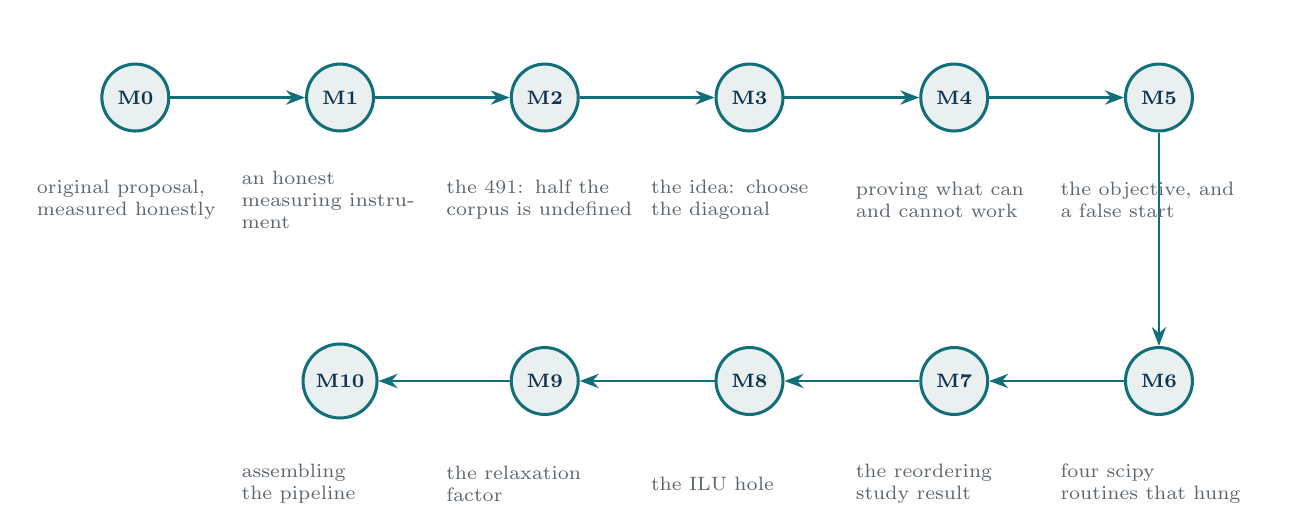
\begin{tikzpicture}[node distance=1.05cm]
  \node[milestone] (m0) at (0,0) {M0};
  \node[milestone] (m1) at (2.6,0) {M1};
  \node[milestone] (m2) at (5.2,0) {M2};
  \node[milestone] (m3) at (7.8,0) {M3};
  \node[milestone] (m4) at (10.4,0) {M4};
  \node[milestone] (m5) at (13.0,0) {M5};
  \node[milestone] (m6) at (13.0,-3.6) {M6};
  \node[milestone] (m7) at (10.4,-3.6) {M7};
  \node[milestone] (m8) at (7.8,-3.6) {M8};
  \node[milestone] (m9) at (5.2,-3.6) {M9};
  \node[milestone] (m10) at (2.6,-3.6) {M10};
  \draw[fl] (m0) -- (m1); \draw[fl] (m1) -- (m2); \draw[fl] (m2) -- (m3);
  \draw[fl] (m3) -- (m4); \draw[fl] (m4) -- (m5); \draw[fl] (m5) -- (m6);
  \draw[fl] (m6) -- (m7); \draw[fl] (m7) -- (m8); \draw[fl] (m8) -- (m9);
  \draw[fl] (m9) -- (m10);
  \node[note,text width=2.5cm] at (0,-1.3) {original proposal,\\measured honestly};
  \node[note,text width=2.5cm] at (2.6,-1.3) {an honest\\measuring instrument};
  \node[note,text width=2.5cm] at (5.2,-1.3) {the 491: half the\\corpus is undefined};
  \node[note,text width=2.5cm] at (7.8,-1.3) {the idea: choose\\the diagonal};
  \node[note,text width=2.5cm] at (10.4,-1.3) {proving what can\\and cannot work};
  \node[note,text width=2.5cm] at (13.0,-1.3) {the objective, and\\a false start};
  \node[note,text width=2.5cm] at (13.0,-4.9) {four scipy\\routines that hung};
  \node[note,text width=2.5cm] at (10.4,-4.9) {the reordering\\study result};
  \node[note,text width=2.5cm] at (7.8,-4.9) {the ILU hole};
  \node[note,text width=2.5cm] at (5.2,-4.9) {the relaxation\\factor};
  \node[note,text width=2.5cm] at (2.6,-4.9) {assembling\\the pipeline};
\end{tikzpicture}}
\caption{The eleven milestones of the project's own contribution, in the order they
actually happened, read left to right along the top row and then left to right again
along the bottom row. Sections~\ref{sec:novel-apk} through~\ref{sec:novel-pipeline} follow
this same order.}
\label{fig:milestones}
\end{figure}

\subsection{Milestone 0: the original proposal, measured honestly}
\label{sec:novel-apk}

Before any of the analysis in this report existed, the group's original course proposal
already contained a candidate for a novel contribution: a rule for choosing a solver based
on one property of the matrix,

\begin{formulabox}
if $A$ is symmetric: use Preconditioned Conjugate Gradient\\
else: use Preconditioned BiCGSTAB
\end{formulabox}

with both branches sharing the same ILU preconditioner. We called this rule APK internally
and it was written up as the project's proposed novelty. When we measured it honestly,
against the actual literature rather than against our own assumptions, this exact rule
turned out to already have a name. It is the default dispatch behaviour described in
Barrett et al.'s \emph{Templates for the Solution of Linear Systems} (SIAM, 1994), and it
is the built-in default in both PETSc and MATLAB's backslash operator. It was not
something we invented; it was something everybody already does.

Worse, when we measured what the rule contributes on top of simply always using
BiCGSTAB, never bothering to check symmetry at all, the answer was close to nothing:

\begin{formulabox}
ILU-Krylov (dispatched):\quad 617 of 736 solved\\
always ILU-BiCGSTAB:\quad\quad\ \ 616 of 736 solved\\
net contribution of the dispatch rule: \textbf{+1 matrix out of 736}
\end{formulabox}

\begin{figure}[H]
\centering
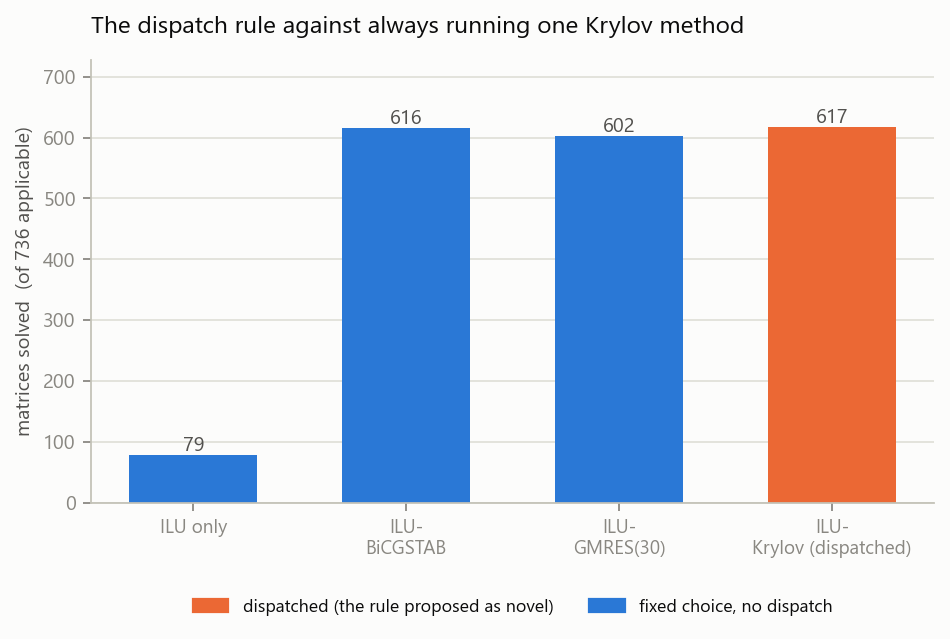
\includegraphics[width=0.78\linewidth]{17_dispatch_ablation.png}
\caption{The symmetry-dispatch rule (APK), measured against always using BiCGSTAB
regardless of symmetry. The entire measured contribution of the rule is one matrix out of
736.}
\label{fig:dispatch-ablation}
\end{figure}

One matrix, out of 736. That number is the reason this project needed an actual new
contribution. The rule is kept in the final benchmark today as \code{ilu\_krylov\_dispatched}
in \code{reference\_solvers.py}, but honestly labelled as a known baseline rather than a
contribution, with a docstring stating plainly what is written above. This was the first
lesson of the entire project, and it set the tone for everything that followed: measure
everything honestly, including your own idea, before claiming it is new. A full,
dedicated treatment of why this rule failed to be novel, and what its measured value
actually is, appears again in Section~\ref{sec:failure-apk}.

\subsection{Milestone 1: building an honest measuring instrument}
\label{sec:novel-harness}

Before any new idea could be tested fairly, the benchmark itself had to be trustworthy,
and the earliest version of the code had several problems, each only found by carefully
auditing its own output rather than trusting it.

A solver's own claim of success was being trusted uncritically: if a routine returned
without raising an exception, it was marked successful, even though some of those runs
had a relative residual as large as $9.71 \times 10^{12}$, wrong by twelve orders of
magnitude. Success rates were divided by the size of the whole corpus, even for methods
such as Conjugate Gradient that are mathematically defined on only a small, symmetric
positive-definite slice of it, which unfairly penalised every specialised method.
Iterative refinement, a technique that polishes an already-computed answer with one
additional cheap step, was being applied to only one method, which is exactly why that
method appeared to be the most accurate; the advantage being measured was the refinement
step, not the method underneath it. Gauss-Seidel and SOR were re-analysing their
triangular system from scratch on every single iteration, up to ten thousand times per
matrix, inflating their measured running time by a factor of eleven to fourteen.

Fixing these was not optional polish; it was the precondition for every later result in
this report to mean anything, and Section~\ref{sec:failure-mistakes} lists all eight
mistakes found this way, not only these four, together with exactly what changed once each
was fixed. The lasting outcome of this milestone is \code{metrics.py}, the single place in
the codebase that decides whether a solve counted as a success, using eight distinct
outcome categories rather than a bare pass or fail, precisely because ``the method could
not even be attempted'' and ``the method was attempted and failed'' are different facts
that a simple binary hides.

\begin{figure}[H]
\centering
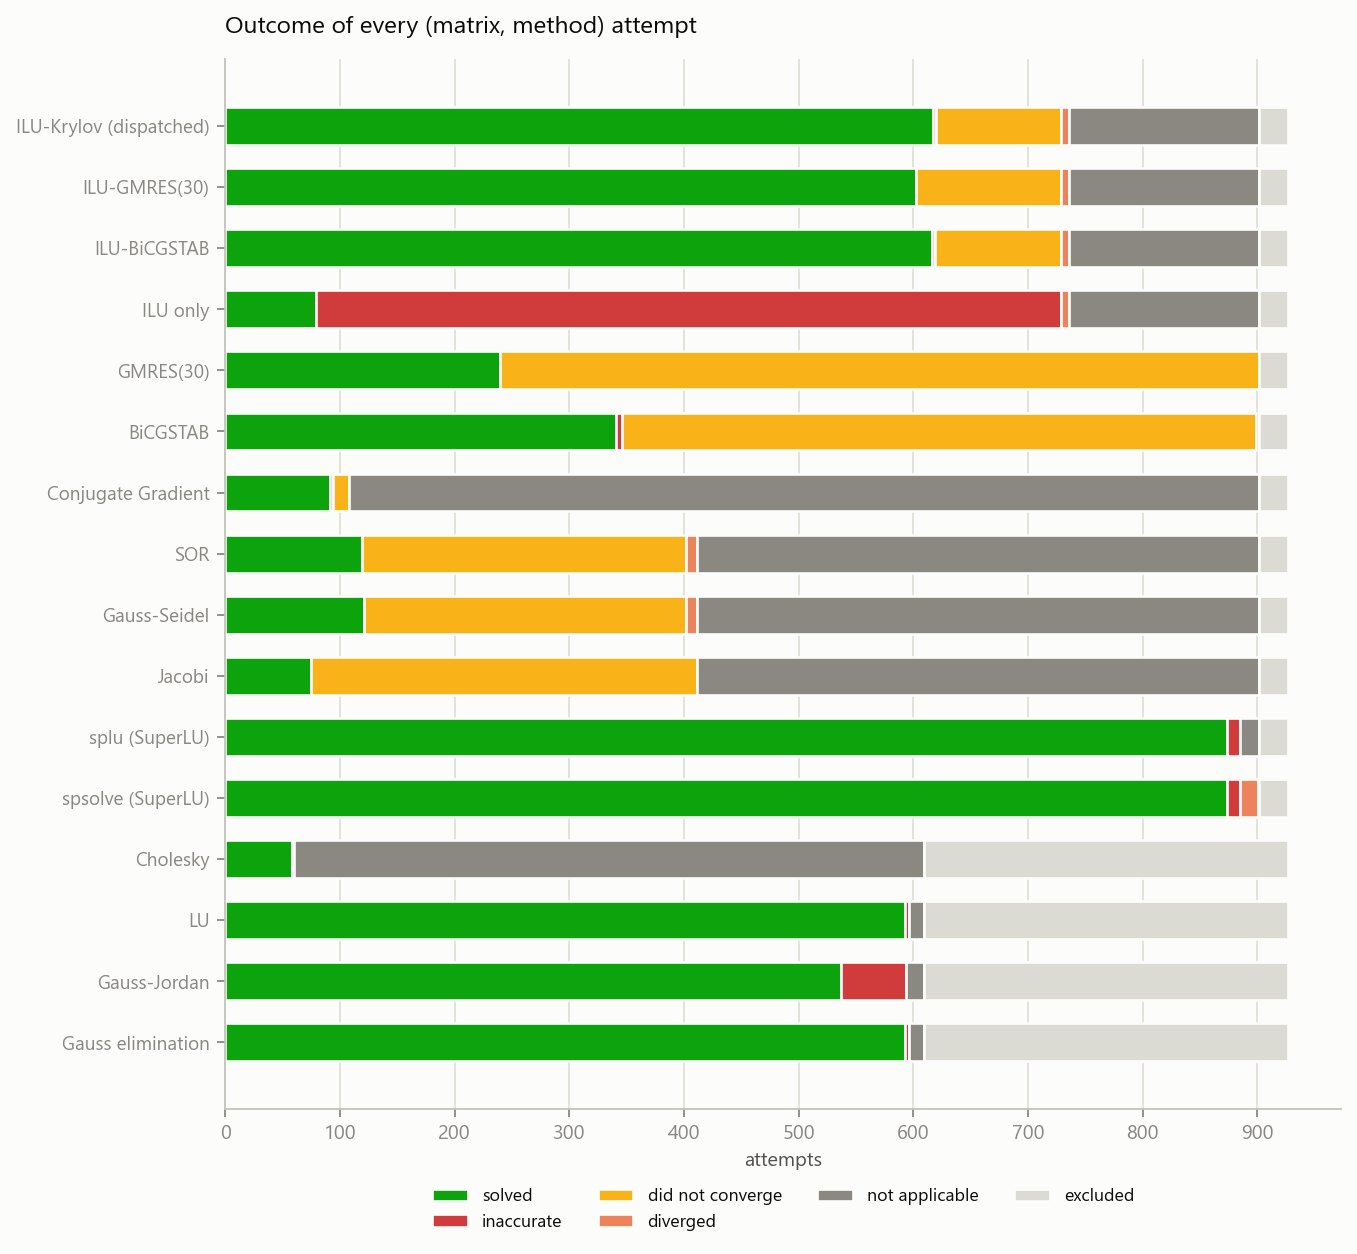
\includegraphics[width=0.82\linewidth]{06_outcomes.png}
\caption{The full breakdown of all 14,832 (matrix, method) attempts across the eight
outcome categories the harness distinguishes. Roughly a quarter of all attempts are
\emph{not\_applicable}, a category that a simple pass/fail measurement would have hidden
inside ``failed.''}
\label{fig:outcomes}
\end{figure}

\subsection{Milestone 2: the discovery that reshaped the project}
\label{sec:novel-491}

Once the harness could be trusted, the first full sweep over the corpus with all sixteen
methods produced one number that reoriented the rest of the project. Jacobi,
Gauss-Seidel, and SOR all divide by the diagonal entries of $A$ at every step, and if even
one diagonal entry is exactly zero, that division is not merely slow or inaccurate; it is
undefined, in exactly the sense that $1/0$ is undefined.

\begin{formulabox}
$$\textbf{491 of 927 matrices (53\%) have at least one zero on the diagonal.}$$
\end{formulabox}

This is the single most consequential fact discovered anywhere in this project. Over half
the corpus was off-limits to Jacobi, Gauss-Seidel, and SOR before a single iteration was
ever attempted, and any comparison that fails to separate ``the method could not even try''
from ``the method tried and failed'' is comparing the wrong things. It is what turned the
project's central question from \emph{is Jacobi slow} into \emph{can Jacobi even be made
applicable in the first place}, a question with a much larger and more tractable answer
space.

\subsection{Milestone 3: the idea, choose the diagonal}
\label{sec:novel-idea}

Once the 491 was understood, an important observation followed almost immediately. The
row order of a matrix is simply a list, row one, row two, row three, decided by whoever
built the matrix, be it a meshing program, a circuit simulator, or an engineer's own
numbering convention, and that order has nothing to do with which solver will later be
applied to it. Crucially, the rows can be reordered without changing the answer at all:
if $P$ is a permutation matrix, then $A\vec{x}=\vec{b}$ if and only if
$(PA)\vec{x} = P\vec{b}$, so permuting rows is completely free with respect to
correctness; it only changes which entries of $A$ end up on the diagonal.

\begin{figure}[H]
\centering
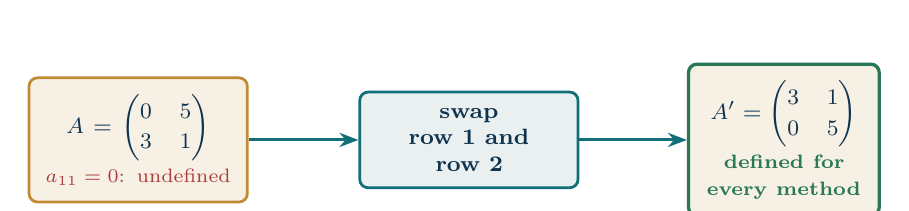
\begin{tikzpicture}
  \node[data] (before) at (0,0) {$\displaystyle A=\begin{pmatrix}0 & 5\\ 3 & 1\end{pmatrix}$\\[2pt]{\scriptsize\color{SBred} $a_{11}=0$: undefined}};
  \node[stage] (arrow) at (4.2,0) {swap\\row 1 and row 2};
  \node[outbox] (after) at (8.2,0) {$\displaystyle A'=\begin{pmatrix}3 & 1\\ 0 & 5\end{pmatrix}$\\[2pt]{\scriptsize\color{SBgreen} defined for every method}};
  \draw[fl] (before) -- (arrow);
  \draw[fl] (arrow) -- (after);
\end{tikzpicture}
\caption{The seed of the entire contribution. Reordering the rows of a matrix changes
nothing about the system it represents, but it changes everything about whether the
stationary methods can even be attempted.}
\label{fig:diagonal-swap}
\end{figure}

Same equations, same answer, completely different eligibility for the stationary methods.
Choosing which row goes where, before the matrix is ever handed to a solver, is the seed
of the entire contribution described in the remainder of this section.

\subsection{Milestone 4: proving what can and cannot work}
\label{sec:novel-proof}

Before searching for a good row order, it was necessary to know which kinds of
preprocessing could possibly help, so the search would not waste effort on something
mathematically pointless. Three candidates were checked, and two were ruled out by direct
algebraic proof rather than trial and error. Scaling every row of $A$ by some factor
leaves Jacobi's iteration matrix $T_J = -D^{-1}(L+U)$ exactly, algebraically unchanged,
because the scaling factor cancels in the formula. Scaling every column is a similarity
transform, and a similarity transform never changes a matrix's eigenvalues, hence never
changes its spectral radius. Symmetric row-and-column permutation, the classical
fill-in-reducing reordering used ahead of direct solvers, was measured directly on real
matrices and barely moved the spectral radius at all, from 0.99012 to 0.99011 in the
fifth decimal place.

Row permutation on its own is the only one of these operations that changes which numbers
sit on the diagonal, and therefore the only one that can change whether Jacobi,
Gauss-Seidel, or SOR are even applicable, let alone how quickly they converge. This proof
is what turned ``try shuffling the rows'' from a guess into a principled, justified
search: the search was restricted to row permutations specifically because it could be
shown that nothing else was worth searching over.

\subsection{Milestone 5: building the objective, and a false start}
\label{sec:novel-objective}

Given that row permutation is the only lever, the next question is which permutation.
There are $n!$ possible orderings for an $n$-row matrix, far too many to try one at a
time, so the choice has to be posed as an optimization problem: pick one entry per row,
and one per column, to occupy the diagonal, an \emph{assignment problem}, which can be
solved exactly rather than approximately.

The existing, industry-standard tool for this is MC64 (Duff and Koster, 1999), which
picks the diagonal maximizing the product of the absolute diagonal values. This is an
excellent objective for direct solvers, since a large diagonal magnitude means the
elimination process is numerically stable, but MC64 was never designed with iterative
convergence in mind: a diagonal entry of size 1{,}000 looks excellent in isolation, but if
the remainder of that row sums to 50{,}000, the row is still poor for Jacobi or
Gauss-Seidel, and MC64 has no way to see that, since it only ever inspects the single
diagonal entry, never the rest of the row.

The objective proposed in this project looks at the whole row instead. For row $i$ with
diagonal candidate $a_{ii}$, define the row ratio

\begin{formulabox}
$$\text{ratio}_i = \frac{\sum_{j \neq i} |a_{ij}|}{|a_{ii}|}$$
\end{formulabox}

A ratio below 1 for every row is exactly the classical condition of strict diagonal
dominance, a sufficient condition that guarantees both Jacobi and Gauss-Seidel converge.
The ratio is therefore not an arbitrary score; it is the precise quantity the classical
convergence theorem is stated in terms of, and this project optimizes it directly, which,
as far as we could determine, nobody had previously done for this specific purpose.
Minimising the worst such ratio across all rows is called the \textbf{bottleneck
objective}, because it is a bottleneck assignment problem, a close relative of MC64's
maximum-weight assignment problem with a different scoring rule.

A second candidate, called \textbf{min-sum}, minimises the total of all the ratios rather
than only the worst one, and was implemented as a natural point of comparison. Working
out the algebra by hand revealed something the group did not expect: since
$1+\text{ratio}_i = (\text{row } i\text{'s total}) / |a_{ii}|$,

\begin{formulabox}
$$\sum_i \log(1+\text{ratio}_i) = \sum_i \log(\text{row totals}) - \sum_i \log|a_{ii}|$$
\end{formulabox}

and the first term on the right does not depend on the permutation at all. Minimising the
left-hand side is therefore exactly the same optimization as maximising
$\sum_i \log|a_{ii}|$, which is precisely MC64's own objective. This was verified directly
on 193 randomly generated matrices: min-sum and MC64 produced an identical objective value
on every single one. Min-sum was not a genuine second alternative; it was MC64 under
another name. This finding is now written permanently into the \code{minsum\_permutation}
function's docstring in \code{reordering.py}, and a dedicated automated test,
\code{test\_minsum\_is\_mc64\_under\_another\_name}, exists specifically so nobody
rediscovers it the hard way. The real competition, in the end, is between two genuinely
different objectives: MC64, the established one, and bottleneck, the one this project
proposes.

\subsection{Milestone 6: four scipy routines that could not be trusted}
\label{sec:novel-hangs}

This milestone cost more real engineering time than any other part of the project, and is
worth recounting in full for what it teaches about trusting a library routine before
measuring it. The first implementation of the bottleneck search used two ready-made scipy
functions built specifically for matching problems of this kind,
\code{min\_weight\_full\_bipartite\_matching} and \code{maximum\_bipartite\_matching}.
Four separate times, in four separate ways, they hung on real matrices from this corpus.

\begin{figure}[H]
\centering
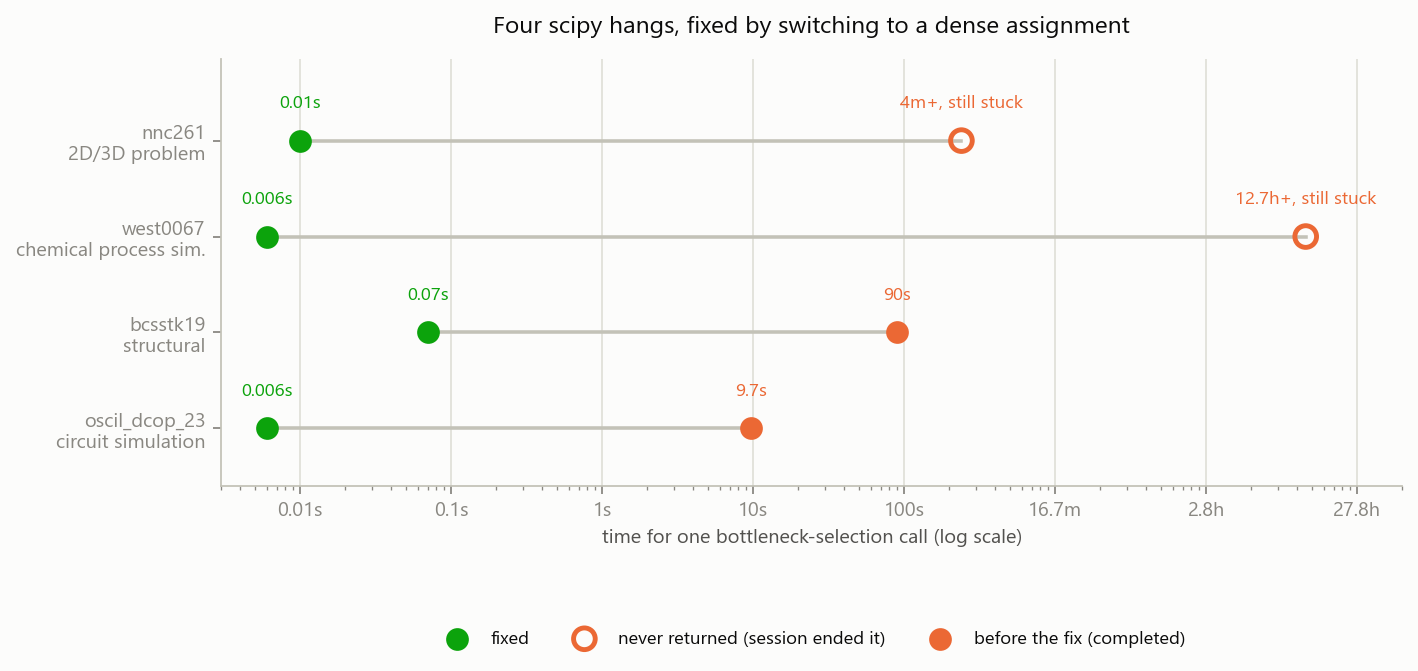
\includegraphics[width=0.82\linewidth]{19_hang_fixes.png}
\caption{The four scipy routine hangs encountered during development, the matrix that
exposed each one, and the wall-clock cost of the fix that replaced the hanging routine
with a dense assignment solve.}
\label{fig:hang-fixes}
\end{figure}

On \code{nnc261}, using raw ratio values as matching weights, the routine had not returned
after 240 seconds. After switching to a numerically safer weight formulation to fix that
first problem, the very same routine hung on a completely different and much smaller
matrix, \code{west0067}, only 67 rows. The other routine, \code{maximum\_bipartite\_matching},
took 7.2 seconds for a single call on \code{bcsstk19}, 817 rows, and the bottleneck search
needs roughly ten such calls per matrix; it was, unhelpfully, slowest exactly when a
matching did exist, the common case. After both original routines were replaced, a
memory-saving size cap meant the largest matrices were still quietly routed through the
same broken code path, and a fourth hang appeared on \code{rw5151}, 5{,}151 rows, caused by
the very safety limit meant to prevent this problem.

The fix, each time, was the same idea: convert the matching problem into a dense
assignment problem and hand it to \code{scipy.optimize.linear\_sum\_assignment}, an
entirely different and, at these matrix sizes, extremely fast and reliable algorithm.
Where the original routines took over ninety seconds or never returned at all, the dense
replacement finished in a fraction of a second, in one measured case more than 1{,}600
times faster. The deeper lesson is that a hang cannot be interrupted from inside a running
program; the only real defence is to test every matrix in the corpus locally before
spending any cloud compute time on it. This is exactly what \code{preflight\_reordering.py}
does: it runs every objective over the entire corpus on an ordinary computer first and
refuses to let anything proceed to the cloud until all 930 matrices pass without a single
hang. The eventual full preflight run completed all 930 matrices in 66.5 minutes with zero
problems, proof that the fix actually worked rather than an assumption that it did.

\subsection{Milestone 7: the reordering study result}
\label{sec:novel-reordering-result}

With the search made reliable, the actual experiment could finally be run: for every
matrix, for each of the three stationary methods, try solving under three conditions, the
row order as given, the row order chosen by MC64, and the row order chosen by this
project's full selector, which computes every candidate diagonal and keeps whichever gives
the smallest estimated $\rho(T_{GS})$.

\begin{formulabox}
systems solved, as given:\quad\ \ 317\\
systems solved, MC64:\quad\quad\ \ 514\\
systems solved, our selector:\quad \textbf{516}\\[4pt]
199 systems rescued in total. Zero lost, since ``change nothing'' is always\\
one of the selector's own candidates.
\end{formulabox}

\begin{figure}[H]
\centering
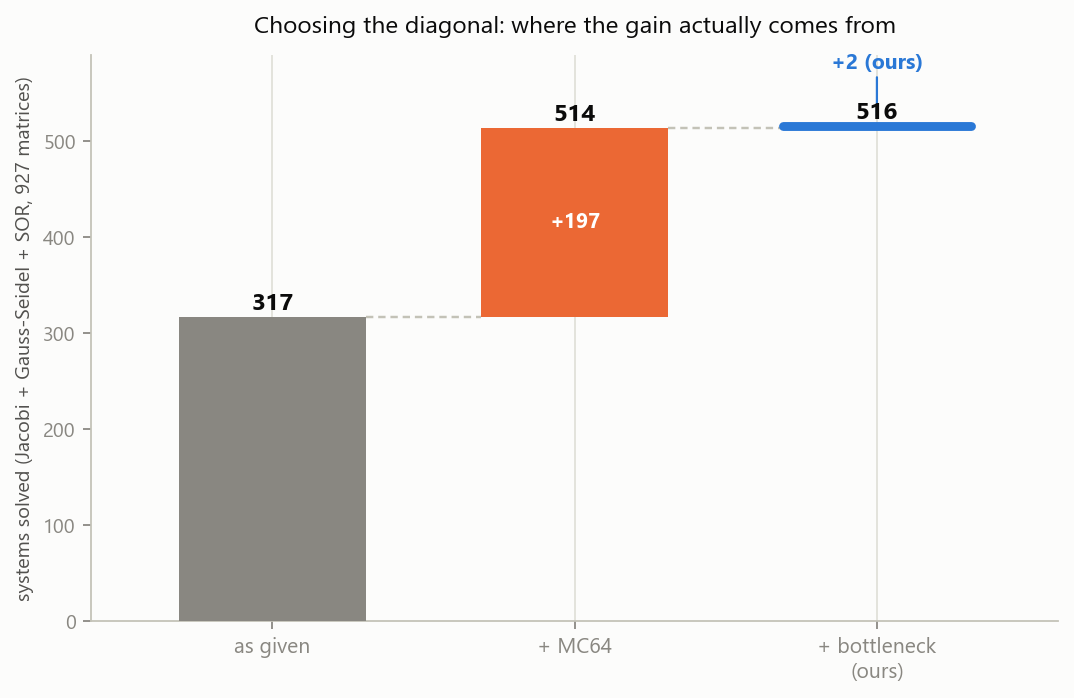
\includegraphics[width=0.82\linewidth]{20_incremental_gains.png}
\caption{Systems recovered, incrementally, as each preprocessing step is added on top of
the previous one, per stationary method.}
\label{fig:incremental-gains}
\end{figure}

Almost all of that gain, however, belongs to MC64, not to the bottleneck idea. Of the 199
rescued systems, 195 are rescued by both objectives together, 4 by bottleneck alone, and 2
by MC64 alone, a net gain for the new objective over the established one of only two
systems. This mirrors Milestone 0 closely: the idea of reordering is genuinely powerful,
but the specific choice of objective barely changes the outcome, at least by this
particular measure. On the quantity bottleneck was actually built to minimise, the worst
row ratio itself rather than the count of systems solved, it wins outright: across the 873
matrices where both objectives produce a finite ratio, bottleneck is strictly better on
367, MC64 is strictly better on precisely 0, and 506 are tied.

\begin{figure}[H]
\centering
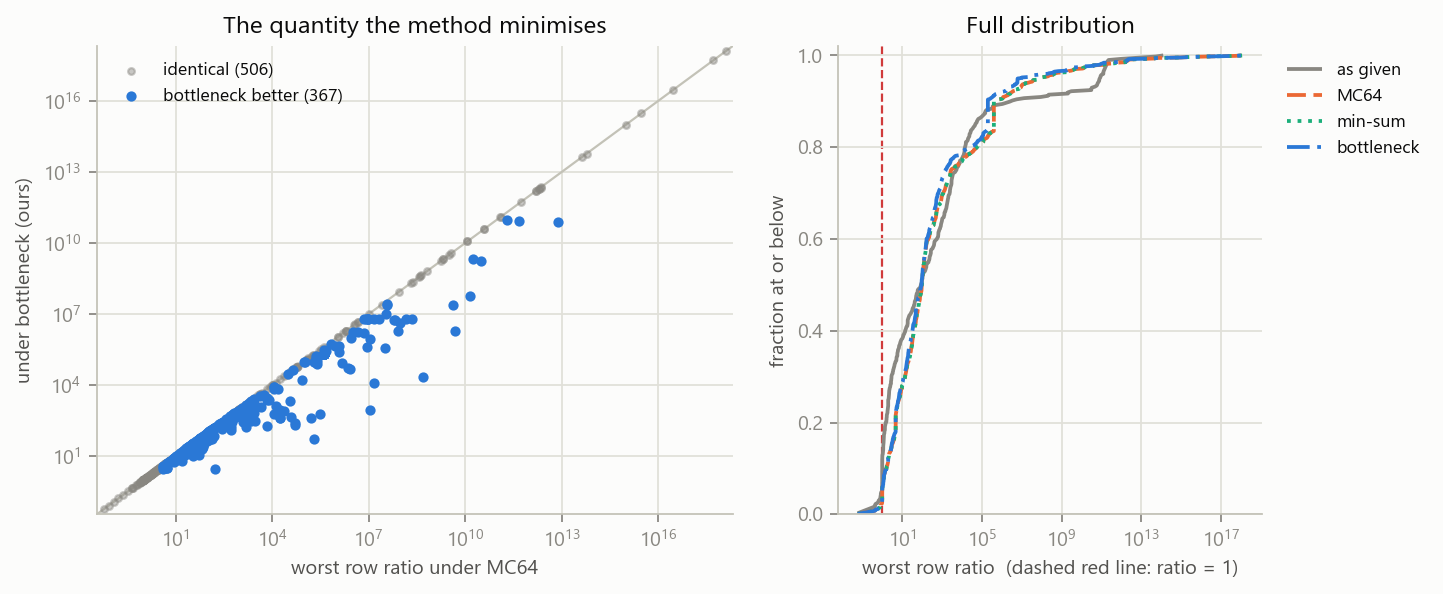
\includegraphics[width=0.7\linewidth]{03_dominance.png}
\caption{Every matrix's worst row ratio under MC64 against the same quantity under
bottleneck. Every point sits on or below the diagonal line; bottleneck never loses on the
quantity it was designed to minimise.}
\label{fig:dominance}
\end{figure}

And the theoretical guarantee the objective was built around, driving the worst row ratio
below 1, turns out to be unreachable on this corpus: 43 matrices were already below the
threshold before any reordering at all, and not one further matrix can be pushed under it
by any row permutation whatsoever. The theorem is true, and, on this data, empty. Why a
result that wins 367 to 0 on its own target quantity converts only two additional systems
is examined directly in Section~\ref{sec:failure-bottleneck}.

\subsection{Milestone 8: the ILU hole}
\label{sec:novel-ilu}

While writing up the reordering result, a related question arose: does the same
zero-on-the-diagonal problem also disable the preconditioned methods, not only the three
stationary ones? The routine that builds an ILU preconditioner tries a proper incomplete
factorization at several settings and, if all fail, falls back to a cruder approximation,
simple diagonal scaling, which also needs a nonzero diagonal, so a zero on the diagonal
closes every door at once, taking the entire preconditioned family down together.

We measured this directly. On the 166 matrices where no ILU preconditioner could be built
at all, BiCGSTAB without a preconditioner solves 12 of them, GMRES(30) solves 11, plain
Gauss-Seidel solves 0, and a sparse direct solver solves 148. That last number is the
important one: it shows these are not intrinsically hard systems, a direct solver handles
nearly all of them without difficulty, they are systems the iterative toolkit specifically
cannot reach, for one narrow and fixable reason. Applying the same diagonal-selection idea
from Milestone 5 in front of ILU, reordering makes \textbf{150 of the 166 constructible},
and of those, 17 actually solve. The gap between 150 buildable and 17 solved is reported
deliberately rather than left implicit: being able to construct a preconditioner is not
the same as the resulting system then converging, a distinction returned to in
Section~\ref{sec:failure-ilu}.

\begin{figure}[H]
\centering
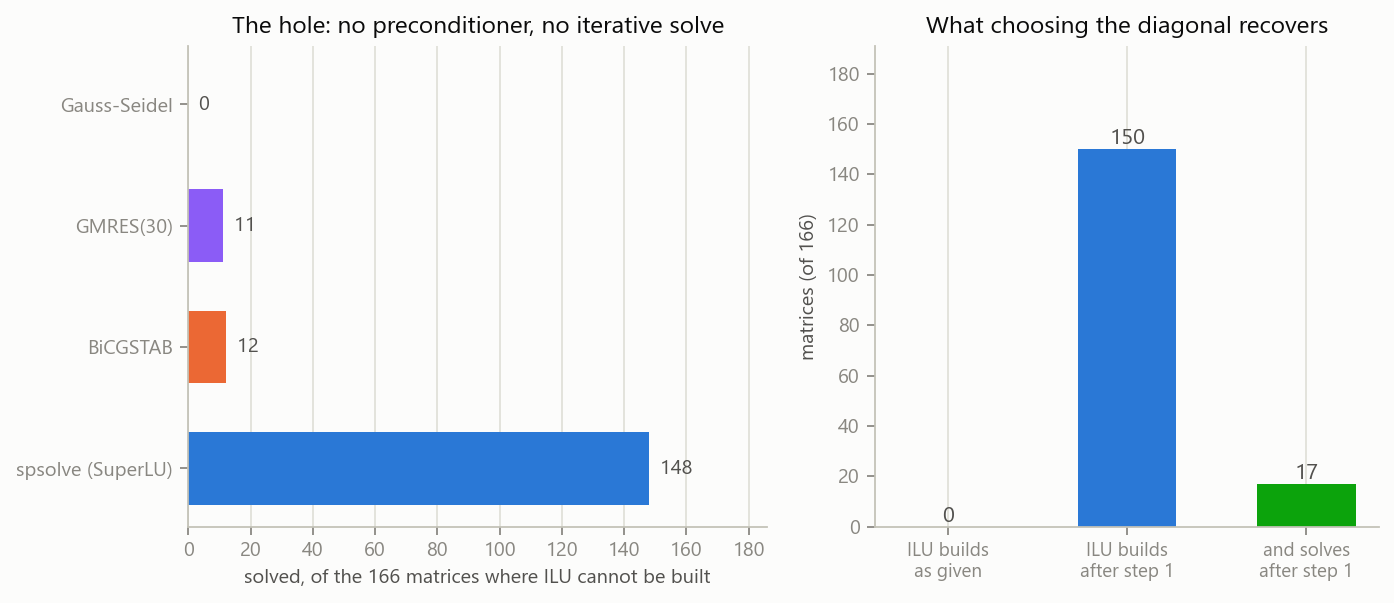
\includegraphics[width=0.86\linewidth]{02_ilu_hole.png}
\caption{Left: which methods can solve the 166 ILU-hole matrices as given. Right: what
reordering recovers once applied in front of ILU construction.}
\label{fig:ilu-hole}
\end{figure}

\subsection{Milestone 9: the relaxation factor, chosen per matrix}
\label{sec:novel-omega}

SOR has one tuning parameter Jacobi and Gauss-Seidel do not: the relaxation factor
$\omega$. Throughout the main sweep, $\omega$ was fixed at 1.25 for every matrix in the
corpus, one number applied uniformly regardless of what the matrix actually looked like.
Measuring whether that fixed choice was even a good idea revealed it was wrong in both
directions at once: plain Gauss-Seidel, equivalent to $\omega=1$, solves 11 systems that
SOR at the fixed $\omega=1.25$ does not, while SOR at $\omega=1.25$ solves 9 systems that
plain Gauss-Seidel does not. Twenty systems in the corpus, in other words, have their
outcome decided entirely by the choice of $\omega$, which is the ceiling of what any
smarter choice could possibly recover.

Young's 1950 formula gives the mathematically optimal relaxation factor from the spectral
radius of the Jacobi iteration matrix:

\begin{formulabox}
$$\omega^{*} = \frac{2}{1+\sqrt{1-\rho(T_J)^2}}$$
\end{formulabox}

\begin{pseudobox}
function ESTIMATE_RHO_JACOBI(A, power_iterations = 60):
    v <- a random unit vector
    for step in 1 .. power_iterations:
        v <- v - (A @ v) / diagonal(A)
        v <- v / norm(v)
    return norm(v)
\vspace{5pt}
function OPTIMAL_OMEGA(rho):
    if rho is not usable, or rho >= 1:
        return 1.0
    return 2 / (1 + sqrt(1 - rho * rho))
\vspace{5pt}
function SOR_ADAPTIVE(A, b, tolerance, max_iterations):
    rho    <- ESTIMATE_RHO_JACOBI(A)
    omega  <- OPTIMAL_OMEGA(rho)
    return SOR(A, b, omega, tolerance, max_iterations)
\end{pseudobox}

$\rho(T_J)$ is estimated cheaply with roughly sixty power-iteration steps and plugged into
Young's formula per matrix, individually, instead of one fixed number for every matrix.
Young's formula is exact only for consistently ordered matrices with property A; most of
this corpus does not belong to that class, so applying the formula anyway is a measured
choice, not an assumed one.

\begin{formulabox}
Gauss-Seidel ($\omega=1$):\quad\quad\quad\ \ 122 solved\\
SOR, fixed $\omega=1.25$:\quad\quad\quad\ 119 solved\\
SOR, $\omega$ chosen per matrix:\quad \textbf{127 solved}
\end{formulabox}

\begin{figure}[H]
\centering
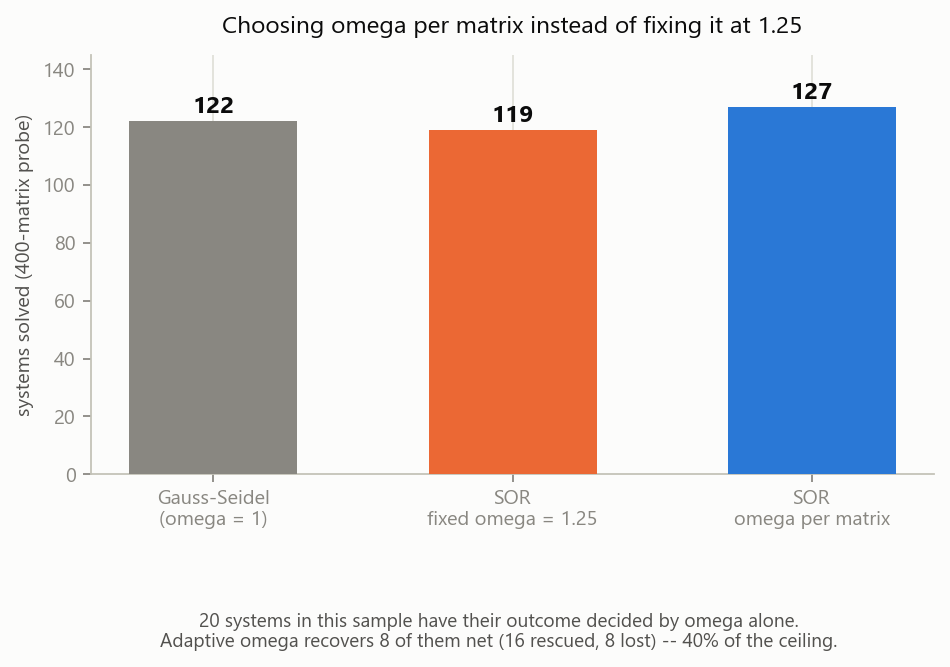
\includegraphics[width=0.7\linewidth]{21_adaptive_omega.png}
\caption{Systems solved by Gauss-Seidel, fixed-$\omega$ SOR, and adaptive-$\omega$ SOR, on
the 400-matrix probe where a usable diagonal exists.}
\label{fig:adaptive-omega}
\end{figure}

Eight net systems recovered out of the twenty-system ceiling identified above, forty
percent of everything that was even possible to gain this way.

\subsection{Milestone 10: assembling the pipeline}
\label{sec:novel-pipeline}

Putting Milestones 7, 8, and 9 together gives the final structure of the contribution: a
two-step preprocessing pipeline that runs in front of an otherwise completely unmodified
solver.

\begin{figure}[H]
\centering
\resizebox{0.98\linewidth}{!}{%
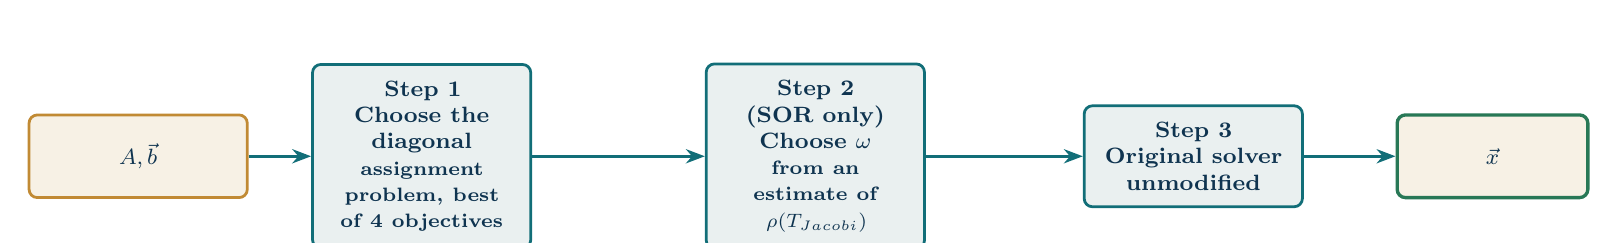
\begin{tikzpicture}
  \node[data] (in) at (0,0) {$A, \vec{b}$};
  \node[stage] (s1) at (3.6,0) {Step 1\\Choose the diagonal\\{\scriptsize assignment problem, best of 4 objectives}};
  \node[stage] (s2) at (8.6,0) {Step 2 (SOR only)\\Choose $\omega$\\{\scriptsize from an estimate of $\rho(T_{Jacobi})$}};
  \node[stage] (s3) at (13.4,0) {Step 3\\Original solver\\\textbf{unmodified}};
  \node[outbox] (out) at (17.2,0) {$\vec{x}$};
  \draw[fl] (in) -- (s1);
  \draw[fl] (s1) -- (s2);
  \draw[fl] (s2) -- (s3);
  \draw[fl] (s3) -- (out);
\end{tikzpicture}}
\caption{The complete preprocessing pipeline, reused here directly from the project's
presentation deck. Steps 1 and 2 never touch the solver itself: $A'\vec{x}=\vec{b}'$
solves the original system exactly, under a relabelling of the rows, so nothing needs to
be undone once the solver returns.}
\label{fig:pipeline}
\end{figure}

Every arm of this pipeline is measured separately as well as together, because ``the
pipeline helps'' is not, by itself, a real result; which specific step helps, and by how
much, is the real result. The full-corpus run measuring every pipeline arm together
completed on all 927 matrices in 413.6 minutes with no hang and no budget stop, and it
confirmed two things that the smaller probes in Milestones 8 and 9 could not show on their
own.

Reordering alone already takes SOR from 119 to 184 (Milestone 7); adding adaptive omega on
top takes it to 208, a 75\% increase over the as-given baseline, stronger than reordering
alone's 55\%. This second step is not loss-free the way the first one is: relative to step
1 alone it gains 36 and loses 12, because there is no ``leave $\omega$ alone'' fallback the
way ``leave the diagonal alone'' is always one of step 1's own candidates.

\begin{figure}[H]
\centering
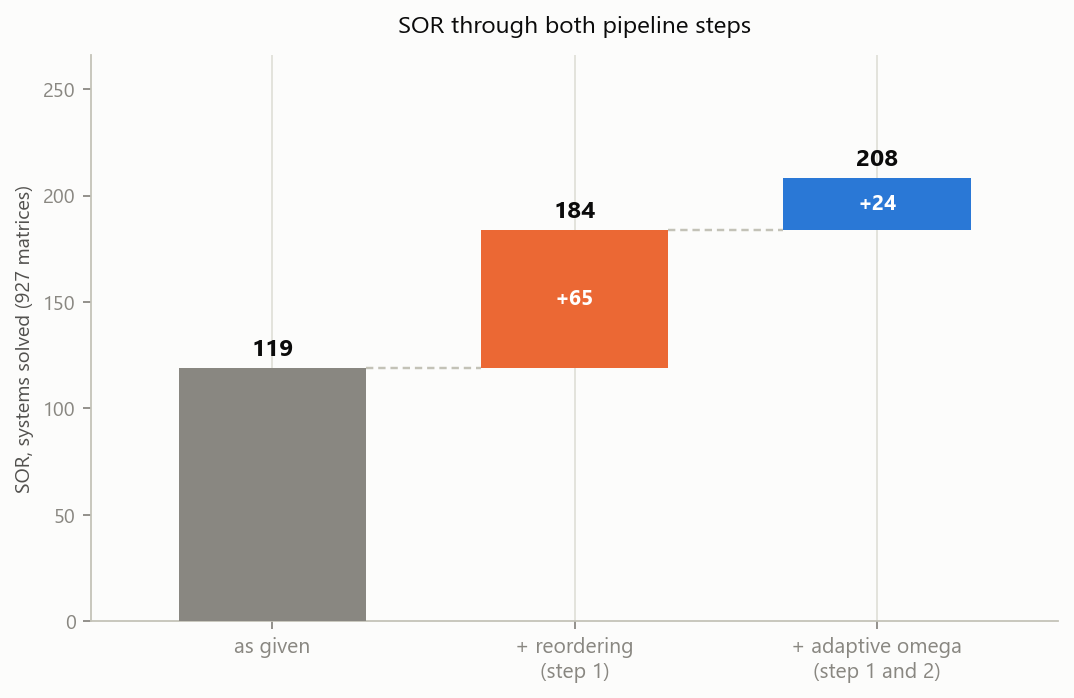
\includegraphics[width=0.6\linewidth]{24_sor_full_pipeline.png}
\caption{SOR solved counts through both pipeline steps, measured on the full 927-matrix
corpus in one run.}
\label{fig:sor-full-pipeline}
\end{figure}

The second confirmation is reordering measured in front of ILU across the entire corpus,
rather than only the 166-matrix subset from Milestone 8, where the baseline could only
ever show a gain since it started at zero. Across all 927 matrices, ILU-BiCGSTAB moves
from 616 to 634 solved, and ILU-Krylov (dispatched) moves from 617 to 635, both on
identical gained-and-lost sets: \textbf{30 gained, 12 lost, net +18}. Twelve matrices
where ILU already worked stop being solvable once the diagonal is reordered, because
reordering changes what the incomplete factorization is built against, and for those
twelve the new factorization is worse. This loss does not appear anywhere in the
166-matrix subset above, because that subset's baseline was zero everywhere; it is the
honest counterpart to Milestone 8's gain, reported here rather than folded silently into
the headline.

\begin{figure}[H]
\centering
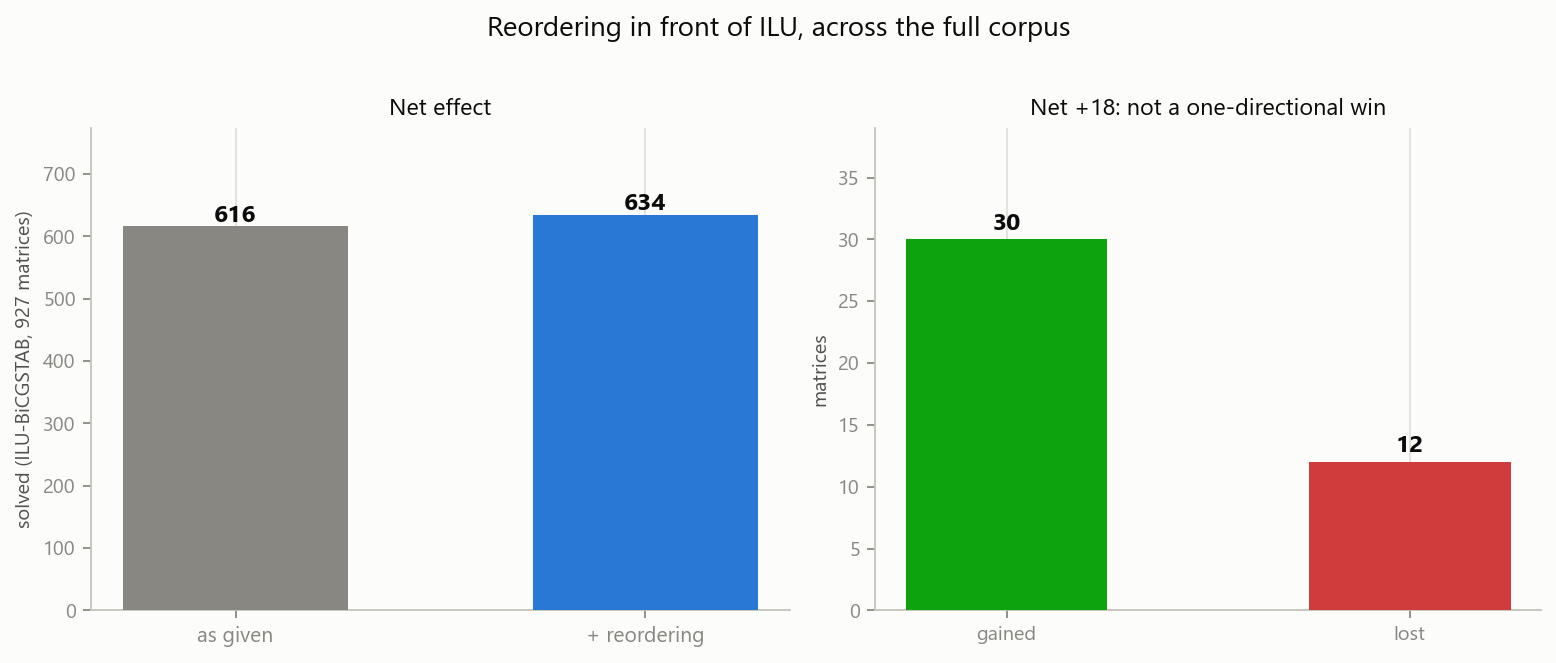
\includegraphics[width=0.86\linewidth]{25_ilu_full_corpus.png}
\caption{Reordering measured in front of ILU across the full 927-matrix corpus, rather
than only the 166-matrix hole. Both ILU-preconditioned methods move on identical
gained-and-lost sets: 30 gained, 12 lost, net +18.}
\label{fig:ilu-full-corpus}
\end{figure}

\clearpage
%============================================================================
\section{Results}
\label{sec:results}

This section reports the measured numbers behind every claim made so far.

\subsection{The headline comparison across sixteen methods}
\label{sec:results-headline}

Table~\ref{tab:headline} reports applicability and conditional success as two separate
numbers for every method, never multiplied together, for the reason given in
Section~\ref{sec:novel-harness}: Conjugate Gradient, for instance, is applicable to only
11.7\% of the corpus, its symmetric positive-definite slice, but solves 84.3\% of what it
is applicable to, a fact a single blended percentage would hide entirely.

\begin{table}[H]
\centering
\caption{Applicability and conditional success for all sixteen methods, corpus of 927
matrices.}
\label{tab:headline}
\small
\begin{tabular}{lrrrr}
\toprule
\hdrow \hdtxt{Method} & \hdtxt{Applicable} & \hdtxt{Solved} & \hdtxt{Applicability} & \hdtxt{Cond. success} \\
\midrule
Gauss elimination & 596 & 593 & 64.3\% & 99.5\% \\
\rowcolor{SBlight} LU & 596 & 593 & 64.3\% & 99.5\% \\
splu (SuperLU) & 885 & 874 & 95.5\% & 98.8\% \\
\rowcolor{SBlight} spsolve (SuperLU) & 901 & 874 & 97.2\% & 97.0\% \\
Cholesky & 60 & 58 & 6.5\% & 96.7\% \\
\rowcolor{SBlight} Gauss-Jordan & 594 & 537 & 64.1\% & 90.4\% \\
Conjugate Gradient & 108 & 91 & 11.7\% & 84.3\% \\
\rowcolor{SBlight} ILU-Krylov (dispatched) & 736 & 617 & 79.4\% & 83.8\% \\
ILU-BiCGSTAB & 736 & 616 & 79.4\% & 83.7\% \\
\rowcolor{SBlight} ILU-GMRES(30) & 736 & 602 & 79.4\% & 81.8\% \\
BiCGSTAB & 902 & 341 & 97.3\% & 37.8\% \\
\rowcolor{SBlight} Gauss-Seidel & 411 & 121 & 44.3\% & 29.4\% \\
SOR ($\omega=1.25$) & 411 & 119 & 44.3\% & 29.0\% \\
\rowcolor{SBlight} GMRES(30) & 902 & 240 & 97.3\% & 26.6\% \\
Jacobi & 411 & 75 & 44.3\% & 18.2\% \\
\rowcolor{SBlight} ILU only & 736 & 79 & 79.4\% & 10.7\% \\
\bottomrule
\end{tabular}
\end{table}

A sparse direct solver wins outright on raw reliability:
\code{spsolve} solves 874 of 927 matrices, against 617 for the best iterative
configuration, a comparison the project's very first, uncorrected sweep never made
available, since applicability and success were still being conflated at that stage.

\begin{figure}[H]
\centering
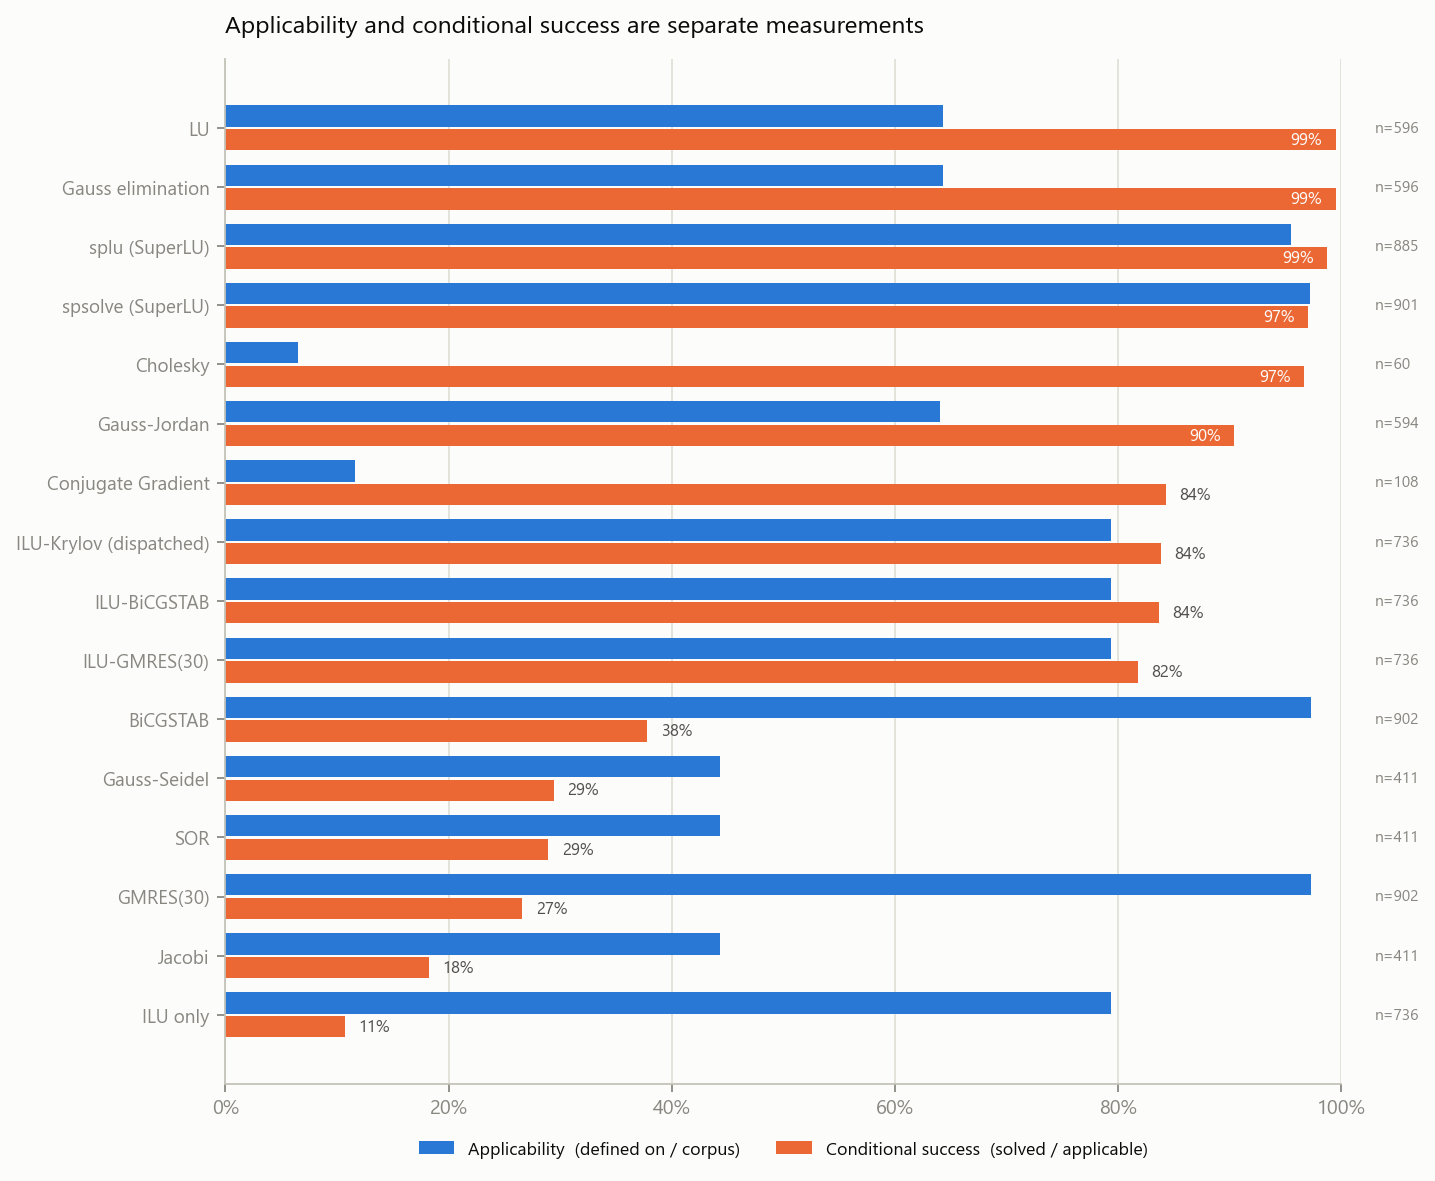
\includegraphics[width=0.85\linewidth]{04_method_scoreboard.png}
\caption{Applicability against conditional success for all sixteen methods. Methods in the
upper right are both broadly applicable and reliable once applicable; ILU-only sits in the
lower right, broadly applicable but rarely successful on its own.}
\label{fig:method-scoreboard}
\end{figure}

\begin{figure}[H]
\centering
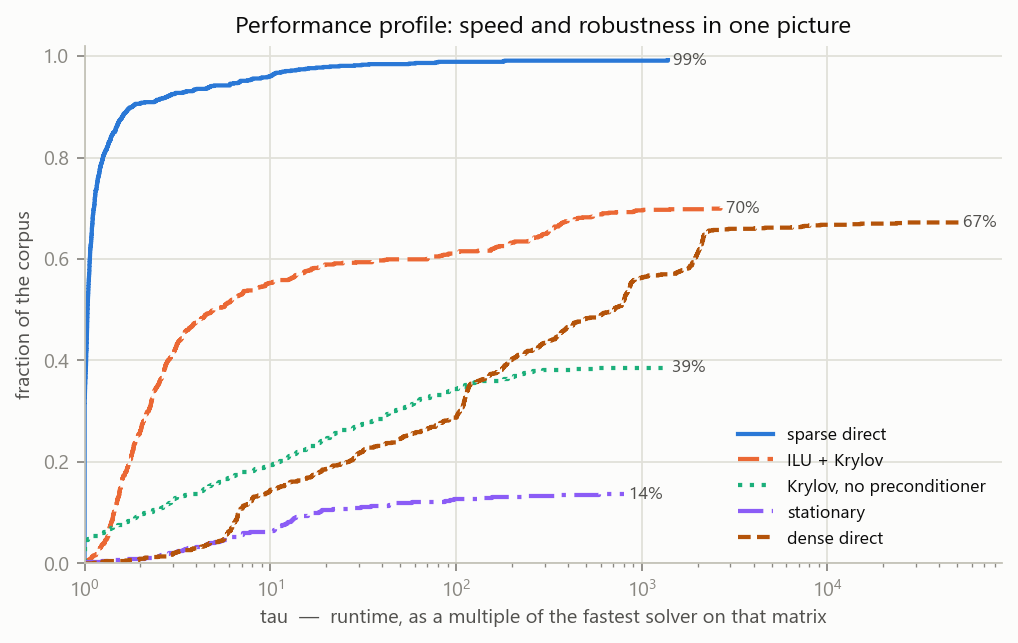
\includegraphics[width=0.85\linewidth]{05_performance_profile.png}
\caption{A performance profile: for each method, how often it is the outright fastest
solver on a matrix it can solve, against how much of the corpus it can solve at all.}
\label{fig:performance-profile}
\end{figure}

\begin{figure}[H]
\centering
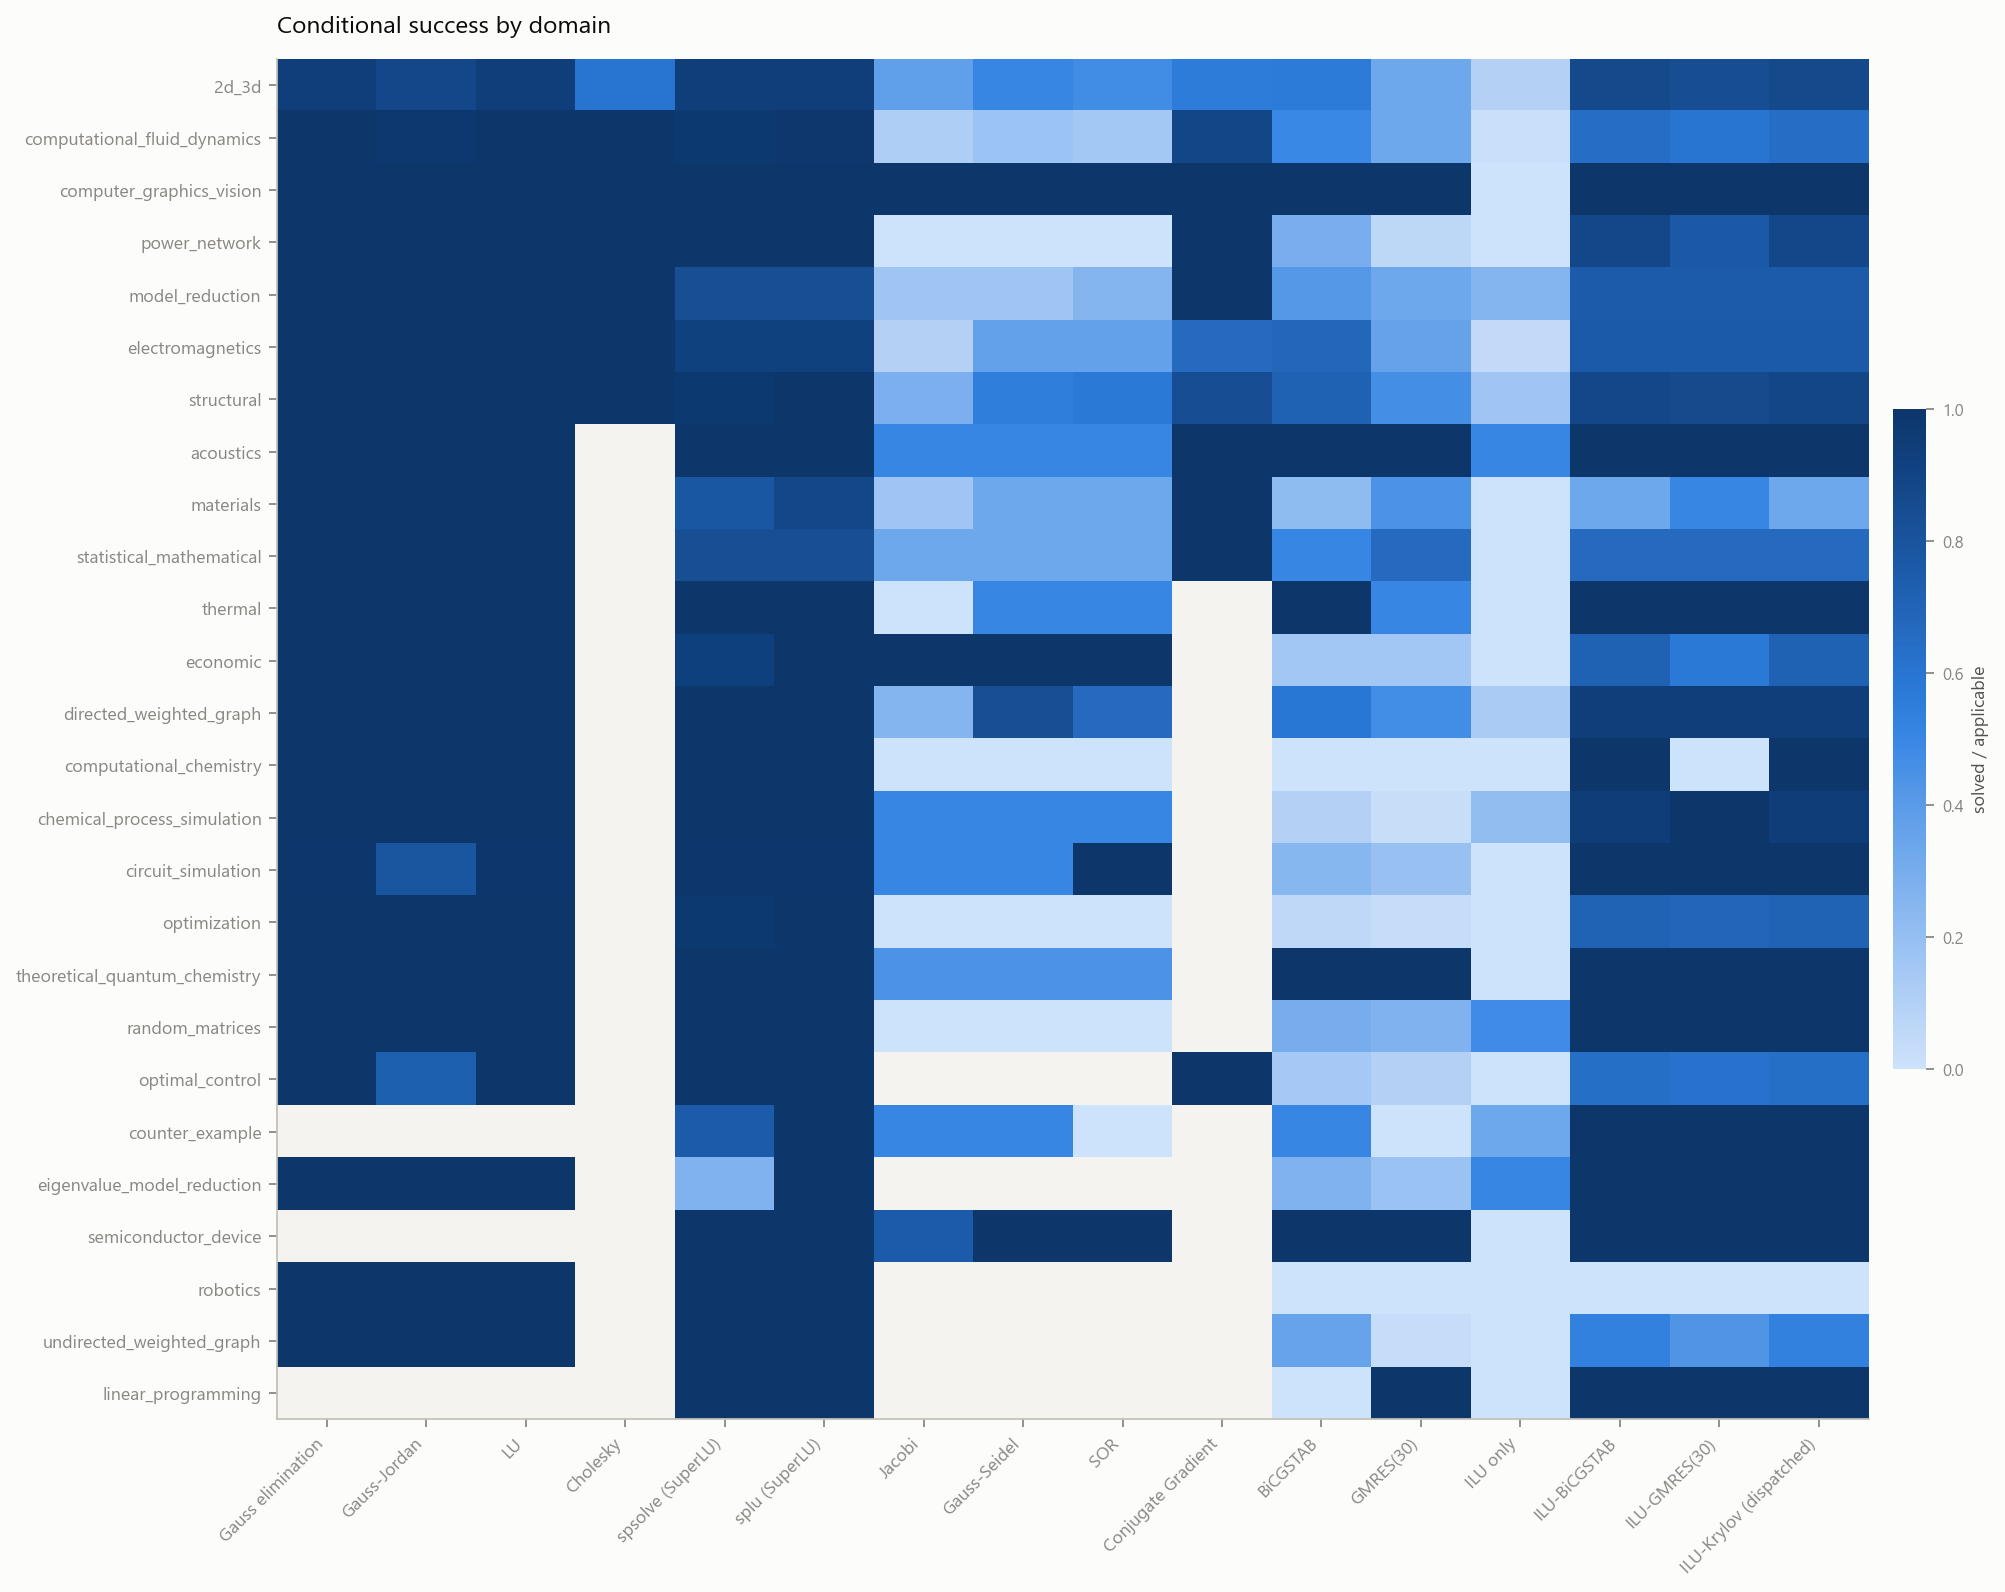
\includegraphics[width=0.85\linewidth]{07_domain_heatmap.png}
\caption{Conditional success rate by method and by domain. Some domains are far friendlier
to the stationary methods than others; circuit-simulation matrices, in particular, are
disproportionately represented among the zero-diagonal failures of Section~\ref{sec:novel-491}.}
\label{fig:domain-heatmap}
\end{figure}

\subsection{Cost and scaling}
\label{sec:results-cost}

Cost is measured in matrix-vector products rather than wall-clock seconds, since shared
cloud hardware timing is not reproducible and iteration counts are not comparable across
methods, one ILU-preconditioned step does the work of many Jacobi steps.

\begin{figure}[H]
\centering
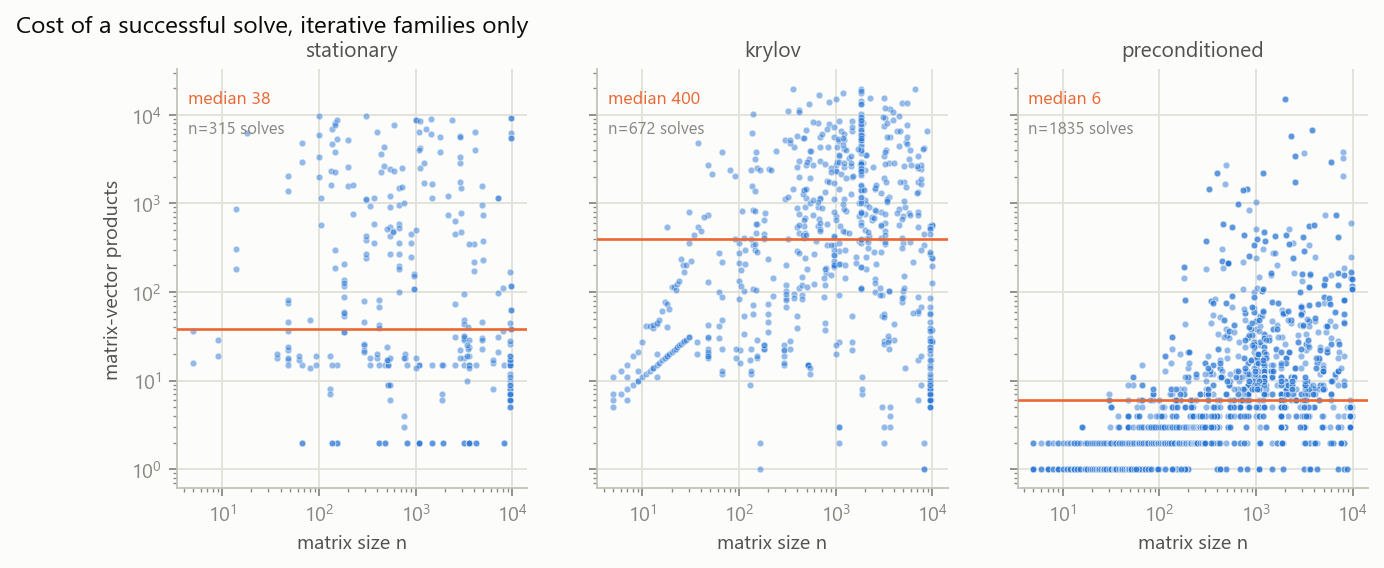
\includegraphics[width=0.82\linewidth]{08_cost_profile.png}
\caption{Cost, in matrix-vector products, for each method's successful solves. Direct
methods pay their entire cost up front; iterative methods trade a larger number of cheap
steps for that same up-front cost.}
\label{fig:cost-profile}
\end{figure}

\begin{figure}[H]
\centering
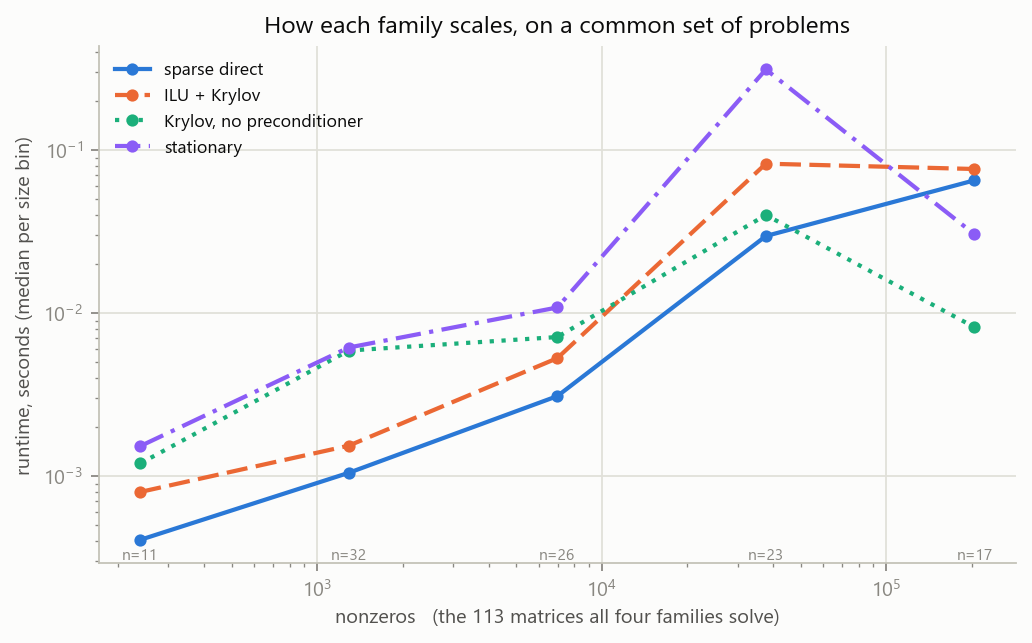
\includegraphics[width=0.82\linewidth]{09_runtime_scaling.png}
\caption{How measured running time grows with matrix size, by method family.}
\label{fig:runtime-scaling}
\end{figure}

\begin{figure}[H]
\centering
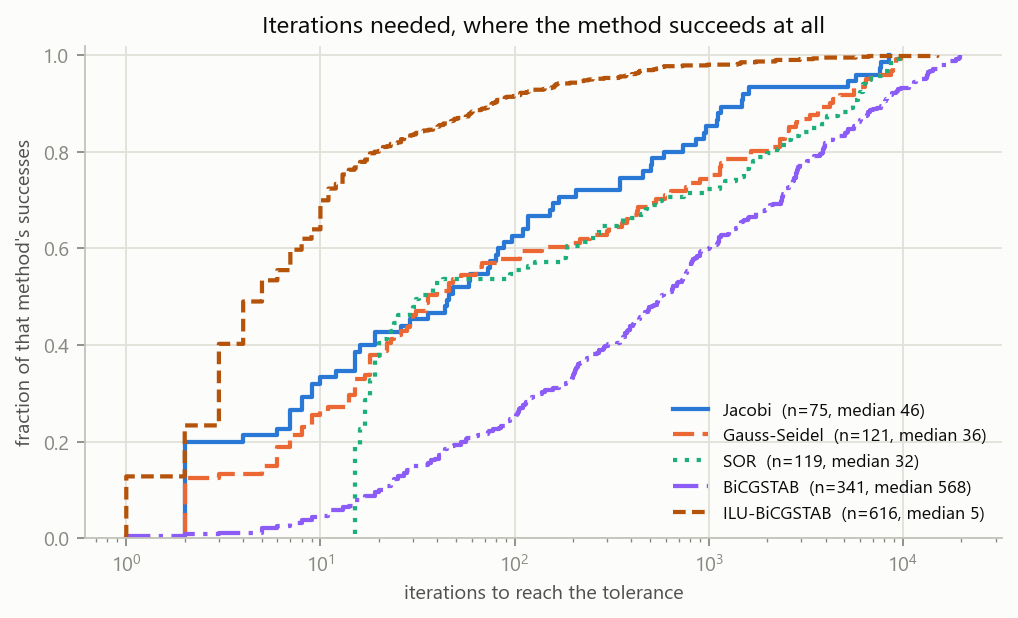
\includegraphics[width=0.82\linewidth]{10_iteration_counts.png}
\caption{Iteration counts needed for convergence, among successful solves, by method.}
\label{fig:iteration-counts}
\end{figure}

\subsection{The base paper's own test, on real data}
\label{sec:results-basepaper}

Restricting to the 411 systems where both Jacobi and Gauss-Seidel are even defined, the
comparison the base paper itself makes looks like this on real data:

\begin{table}[H]
\centering
\caption{Convergence outcomes for Jacobi and Gauss-Seidel, restricted to the 411 systems
where both are applicable.}
\label{tab:basepaper}
\small
\begin{tabular}{lr}
\toprule
\hdrow \hdtxt{Outcome} & \hdtxt{Count} \\
\midrule
Both converge & 75 \\
\rowcolor{SBlight} Only Gauss-Seidel converges & 46 \\
Only Jacobi converges & 0 \\
\rowcolor{SBlight} Neither converges & 293 \\
\bottomrule
\end{tabular}
\end{table}

Khrapov and Volkov report 1{,}095 only-Jacobi cases among their own random matrices at $n
\leq 5$; on this corpus, at realistic sizes, that case never once occurs. On the 100
self-generated random matrices built specifically to reproduce the base paper's own
validation approach at larger scale, the picture is starker still: neither Jacobi nor
Gauss-Seidel solves a single one of the 100, while a direct solver solves all 100, and the
spectral radius of the random-matrix iteration matrices grows roughly in proportion to
matrix size, so the paper's own validation method stops working almost as soon as the
matrices are made larger than the paper itself tested.

\begin{figure}[H]
\centering
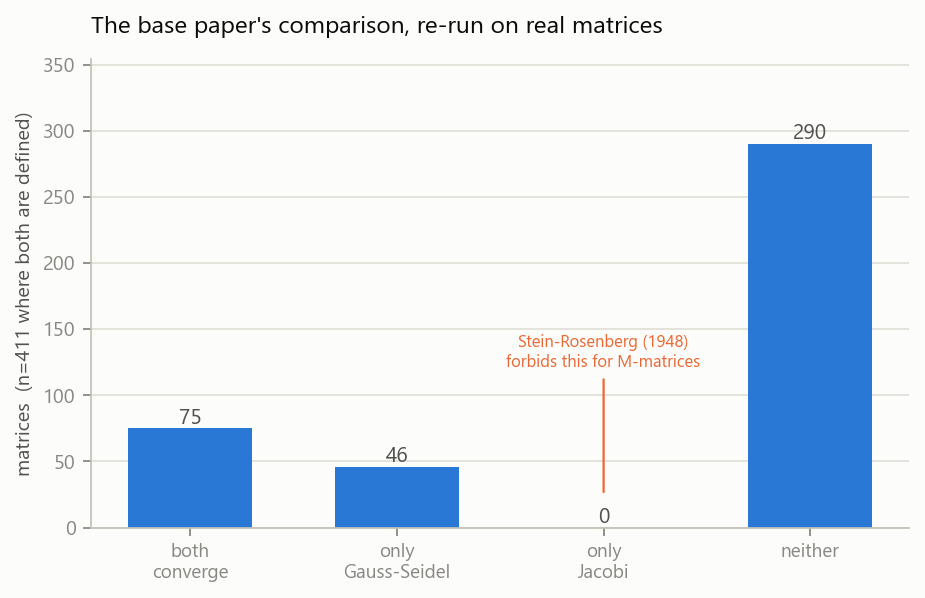
\includegraphics[width=0.82\linewidth]{14_jacobi_vs_gauss_seidel.png}
\caption{The base paper's own question, Jacobi against Gauss-Seidel, answered on real
matrices rather than random ones.}
\label{fig:jacobi-vs-gs}
\end{figure}

\subsection{Spectral prediction, validated}
\label{sec:results-spectral}

The textbook criterion, $\rho(T) < 1$ implies convergence, agrees with the actually
observed outcome on 99.3\% of Jacobi attempts and 98.2\% of Gauss-Seidel attempts across
the 905 matrices where the spectral radius could be computed exactly. The one Jacobi
disagreement worth naming individually is \code{cdde6}, already introduced in
Section~\ref{sec:datasets-examples}: $\rho(T_J)=0.717$, provably convergent, yet the
residual peaks at 44{,}764 times its starting value at iteration 73 before converging at
iteration 178, a transient large enough that an overly strict divergence guard could
mistake it for genuine divergence. Once this single case is accounted for, the theory's
\code{converges} prediction for Jacobi is correct on all 71 of 71 cases it applies to.

\begin{figure}[H]
\centering
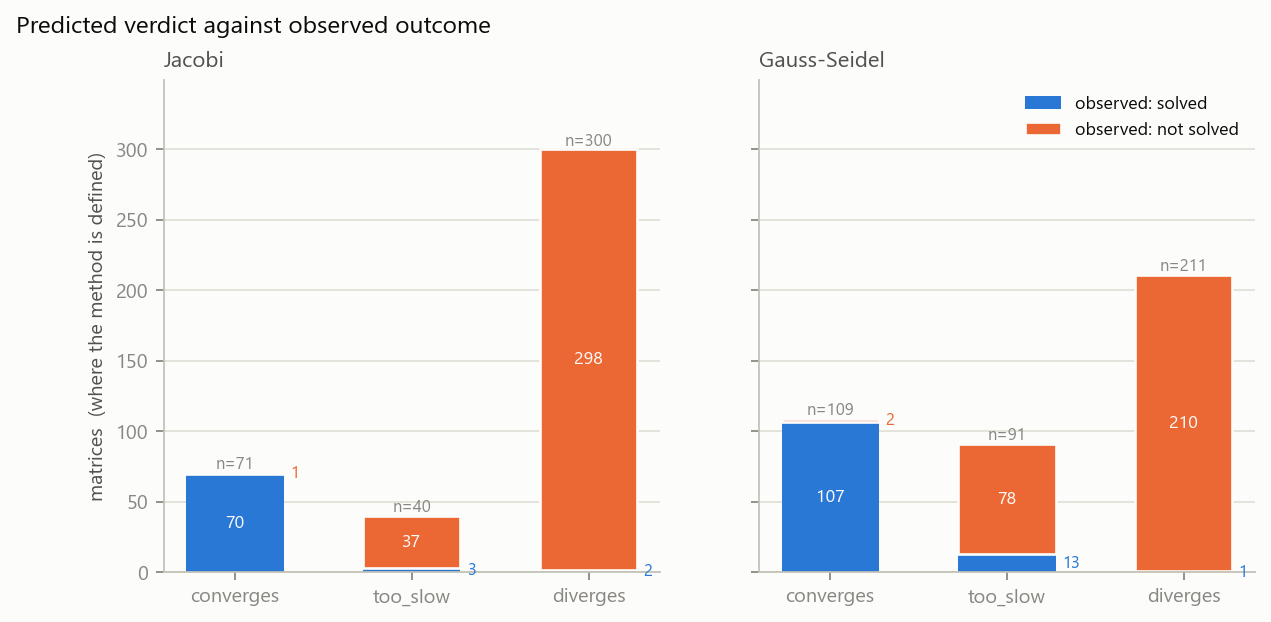
\includegraphics[width=0.82\linewidth]{13_prediction_vs_observation.png}
\caption{Predicted convergence from the spectral radius against the observed outcome, for
Jacobi and Gauss-Seidel.}
\label{fig:prediction-vs-observation}
\end{figure}

\subsection{Refinement, given to every method}
\label{sec:results-refinement}

Applying one pass of iterative refinement identically to every method, rather than to a
single favoured one as in the earliest version of this project, changes the accuracy
ranking outright: Jacobi's median relative forward error falls from $1.893\times10^{-8}$
to $6.985\times10^{-16}$, making it, after refinement, the single most accurate method in
the entire benchmark, a factor of one hundred better than the dispatched ILU method's
$7.111\times10^{-14}$. This comes at a real cost in matrix-vector products, 59 without
refinement against 279 with one pass, a cost that would have been invisible under the
earliest version of the harness, which measured accuracy for one method at a time rather
than as an orthogonal, universally applied factor.

\begin{figure}[H]
\centering
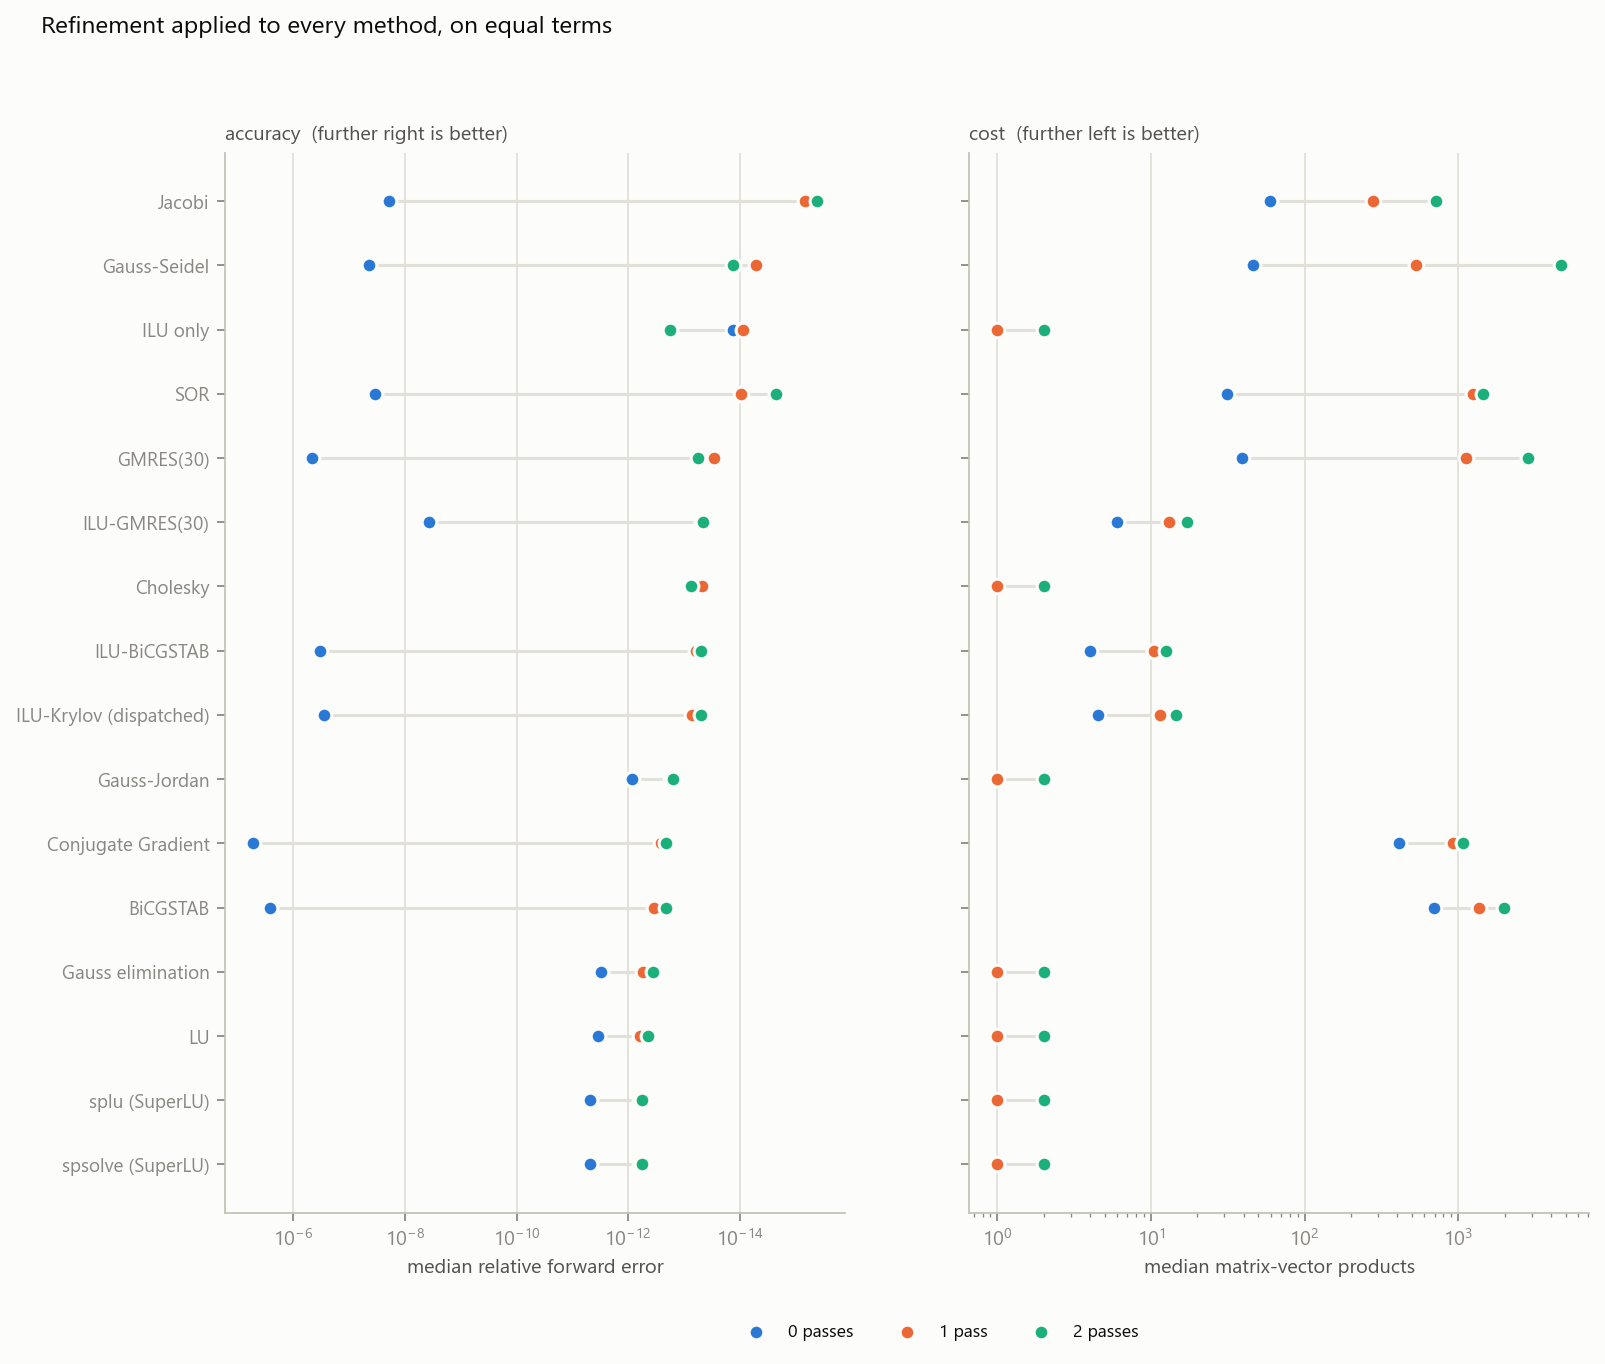
\includegraphics[width=0.82\linewidth]{15_refinement_effect.png}
\caption{Median relative forward error at zero, one, and two refinement passes, by
method.}
\label{fig:refinement-effect}
\end{figure}

\begin{figure}[H]
\centering
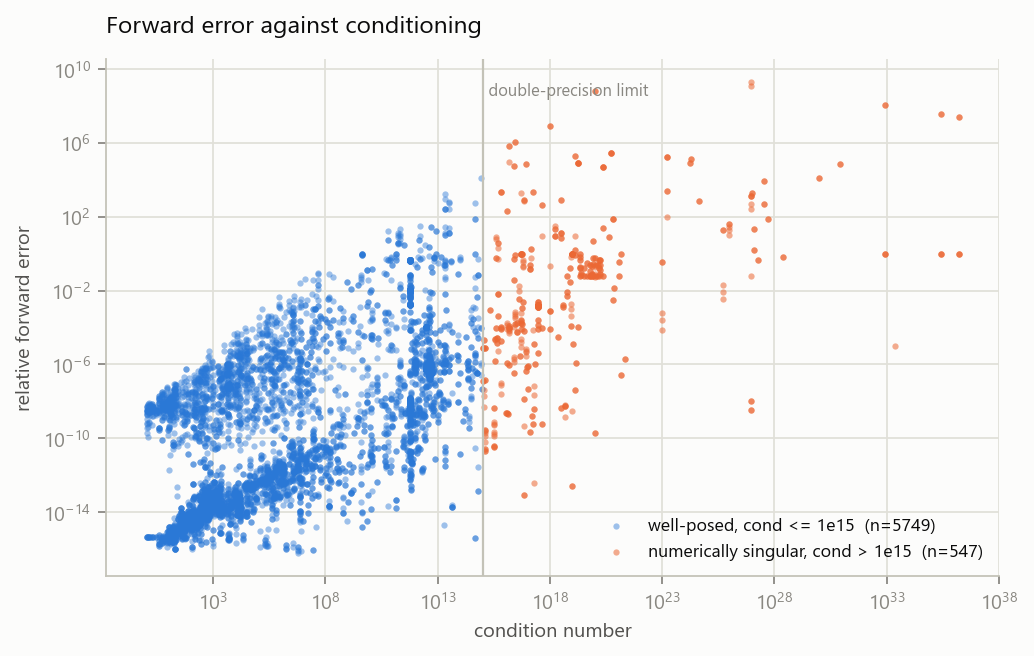
\includegraphics[width=0.7\linewidth]{16_conditioning.png}
\caption{Accuracy, split by whether the underlying matrix is numerically ill-conditioned,
across methods.}
\label{fig:conditioning}
\end{figure}

\subsection{The reordering pipeline, on the stationary methods}
\label{sec:results-pipeline}

The headline contribution of this project, restricted to the parts that do not touch ILU
construction, is a preprocessing pipeline that raises the success rate of the three
stationary solvers substantially, with every gain measured on the same run as its own
baseline.

\begin{table}[H]
\centering
\caption{Systems solved by each stationary method, as given and with the full
preprocessing pipeline, 927-matrix corpus.}
\label{tab:pipeline-headline}
\small
\begin{tabular}{lrrr}
\toprule
\hdrow \hdtxt{Method} & \hdtxt{As given} & \hdtxt{With pipeline} & \hdtxt{Change} \\
\midrule
Jacobi & 76 & 124 & +63\% \\
\rowcolor{SBlight} Gauss-Seidel & 122 & 208 & +70\% \\
SOR & 119 & 184 & +55\% \\
\bottomrule
\end{tabular}
\end{table}

\begin{figure}[H]
\centering
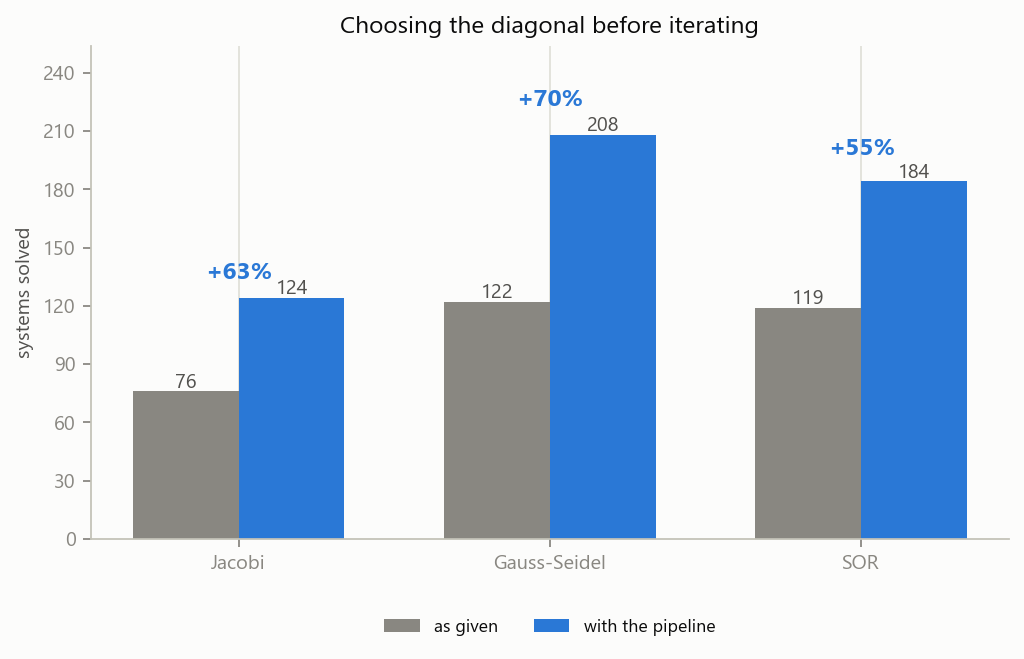
\includegraphics[width=0.82\linewidth]{01_pipeline_scoreboard.png}
\caption{The headline pipeline result: systems solved as given against systems solved with
the full pipeline, per stationary method, with the percentage gain printed above each
pair.}
\label{fig:pipeline-scoreboard}
\end{figure}

One hundred ninety-nine systems recovered in total, none lost, since the selector
described in Section~\ref{sec:novel-objective} always includes ``change nothing'' among
its own candidates and so can never score worse than doing nothing at all. Why the
project's own bottleneck objective, despite winning decisively on the quantity it targets,
contributes only a small share of that recovery over the established MC64 baseline is
examined directly in the failure analysis that follows.

\clearpage
%============================================================================
\section{Failure Analysis}
\label{sec:failure}

Our course teacher specifically asked for a dedicated treatment of why a given solver
fails, and why, together with what novel remedy was proposed in response, for both the
classical methods from the base paper and the methods this project designed itself, even
where some of this ground has already been touched on earlier in the report. This section
is that treatment, gathered in one place. It is organised as a sequence of specific
failures, each stated as plainly as we could manage: what failed, why it failed, what we
tried in response, and, where a remedy exists, how much of the failure it actually closes.
Two of the entries below are failures of the project's own methodology, not of a solver,
because an honest failure analysis of this project has to include the mistakes the
project itself made, not only the mistakes made by the matrices it was testing.

\subsection{Why Jacobi, Gauss-Seidel, and SOR fail: undefined before they start}
\label{sec:failure-undefined}

The most basic failure mode of the three classical stationary methods on this corpus is
not slowness or inaccuracy; it is that the method cannot be attempted at all.
Section~\ref{sec:novel-491} already established the mechanism: each method divides by the
diagonal entries of $A$, and 491 of 927 matrices, 53\% of the corpus, carry at least one
zero on that diagonal. This is a structural failure, decided entirely by which row of the
matrix happened to be listed as which row, an accident of the software that produced the
matrix rather than any property of the underlying physical system. The remedy this project
designed in response is the diagonal-selection pipeline of
Section~\ref{sec:novel-objective}, and a perfect matching over the nonzero entries of $A$
supplies a usable diagonal whenever one exists at all, which is why this specific failure
mode, unlike the one in the next subsection, is one the pipeline can address directly
rather than only partially.

\subsection{Why they still fail when defined: the theorem wall}
\label{sec:failure-theorem-wall}

The remaining failure mode is harder, and it applies even to matrices where the diagonal
was never a problem. Table~\ref{tab:theorem-wall} sorts every matrix with a computable
spectral radius into the classical hypothesis class it satisfies (a matrix that meets more
than one class is credited to the strongest one that applies) and reports the observed
success rate of Jacobi and Gauss-Seidel inside each class.

\begin{table}[H]
\centering
\caption{Success rate by classical hypothesis class, across the 905 matrices with a
computable spectral radius.}
\label{tab:theorem-wall}
\small
\begin{tabular}{lrrr}
\toprule
\hdrow \hdtxt{Class} & \hdtxt{Matrices} & \hdtxt{Jacobi converges} & \hdtxt{Gauss-Seidel converges} \\
\midrule
Strictly diagonally dominant & 43 & 88.4\% & 88.4\% \\
\rowcolor{SBlight} H-matrix & 83 & 77.1\% & 80.7\% \\
M-matrix & 34 & 64.7\% & 76.5\% \\
\rowcolor{SBlight} Symmetric positive definite & 101 & 27.7\% & 51.5\% \\
\textbf{No theorem applies} & \textbf{192} & \textbf{1.6\%} & \textbf{9.9\%} \\
\bottomrule
\end{tabular}
\end{table}

\begin{figure}[H]
\centering
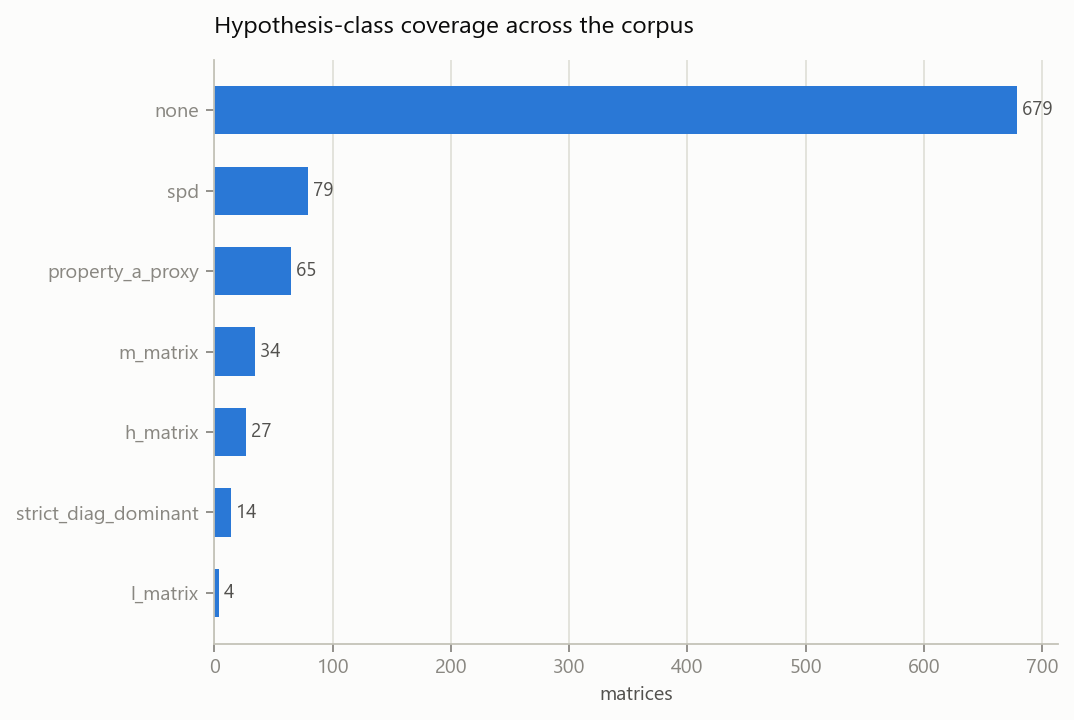
\includegraphics[width=0.82\linewidth]{12_hypothesis_coverage.png}
\caption{How many corpus matrices fall under each classical convergence-guarantee
hypothesis, reused from Section~\ref{sec:methods-spectral}. The class sizes here are what
Table~\ref{tab:theorem-wall} reports a success rate against.}
\label{fig:theorem-wall}
\end{figure}

Where a classical theorem applies at all, Jacobi works 65 to 88\% of the time; where none
applies, 1.6\%. Of the 75 systems where both Jacobi and Gauss-Seidel converge, 72, or 96\%,
are covered by some classical class, against a base rate of 53.6\% across the applicable
set. The theorems are never wrong, they simply do not reach most of the corpus: coverage
across the 905 analysed matrices is none for 680 of them, symmetric positive definite for
81, the property-A proxy for 65, M-matrix for 34, H-matrix for 27, strictly diagonally
dominant for 14, and L-matrix for 4.

The Householder-John theorem, which guarantees Gauss-Seidel convergence on symmetric
positive-definite matrices, is a sharp illustration of exactly this gap. On the 104 real
SPD systems in the corpus, $\rho(T_{GS}) < 1$ holds on 98 of them, confirming the theorem
outright. Within a ten-thousand-iteration budget, though, it only delivers a solved system
on 44. The other 54 sit at $\rho(T_{GS})$ between 0.9984 and 1.0 (never reaching it), with
a median iteration count to convergence of 1{,}798{,}184 and a maximum beyond
$9.9\times10^{13}$. The theorem is true and, for practical purposes on more than half its
own guaranteed population, useless. This gap between converges and converges usefully,
first introduced in Section~\ref{sec:methods-spectral}, is what defeats every
permutation-based remedy attempted in this project, as the next subsections show in turn.

\subsection{Why the original novel proposal, APK, was not novel}
\label{sec:failure-apk}

Section~\ref{sec:novel-apk} already told the story; this subsection states its failure
mode plainly, as the failure analysis this section was asked to provide. The rule failed
to be a contribution for two independent reasons, and it is worth separating them because
they call for different lessons. First, it failed a literature check: symmetry-dispatched
preconditioned Krylov selection is the documented default behaviour in Barrett et al.'s
\emph{Templates} (1994) and the built-in default in both PETSc and MATLAB, so the rule was
not new regardless of how it performed. Second, and independently, it failed a measurement
check: even judged purely on its own merits, ignoring the literature entirely, it
contributes one solved matrix out of 736 over the naive baseline of always choosing
BiCGSTAB. Either failure alone would have been enough to disqualify it as a contribution;
having both at once removed any ambiguity. The remedy was not a fix to the rule; it was
demoting the rule to an honestly labelled baseline and building an actual new objective,
described starting in Section~\ref{sec:novel-idea}, in its place. The lesson this failure
taught, that every later milestone in this project tried to apply, is to check both the
literature and the measured effect size before calling anything novel.

\subsection{Why the first benchmark harness produced false results}
\label{sec:failure-mistakes}

A benchmark that lies to itself before any solver is even compared is a different kind of
failure from a solver that fails on a hard matrix, but it is no less important to a
failure analysis, since every later result in this report depends on this one having been
caught and fixed. Table~\ref{tab:mistakes} lists all eight defects found in the earliest
version of the project's own measuring instrument, each one changing a headline number
once corrected.

\begin{table}[H]
\centering
\caption{Eight methodological defects found in the project's own harness, and their
measured effect once fixed.}
\label{tab:mistakes}
\small
\begin{tabularx}{\linewidth}{p{4.6cm}X}
\toprule
\hdrow \hdtxt{Defect} & \hdtxt{Effect of the fix} \\
\midrule
Trusted a solver's own success flag & 57 false successes caught, one with relative
residual $9.71\times10^{12}$ \\
\rowcolor{SBlight} Divided success by the whole corpus & Conjugate Gradient's true
conditional success rose from a reported 10.4\% to 84.3\% \\
Refinement given to one method only & Accuracy is now an orthogonal, universally applied
factor (Section~\ref{sec:results-refinement}) \\
\rowcolor{SBlight} Re-factored inside the iteration loop & Gauss-Seidel and SOR runtime
fell by a factor of 11 to 14 \\
An overly strict divergence guard & \code{cdde6} and similar non-normal cases (peak
44,764$\times$) were being wrongly recorded as divergent \\
\rowcolor{SBlight} Two copies of the library drifting apart & Notebooks are now generated,
never hand-edited, and the accidental copy removed from the repository \\
Downloaded files never verified against their own header & Six truncated files
(Section~\ref{sec:datasets-bookkeeping}) caught before silently corrupting a run \\
\rowcolor{SBlight} Trusted two scipy routines without local testing & The four hangs of
Section~\ref{sec:novel-hangs}, one costing an entire twelve-hour cloud session before being
traced \\
\bottomrule
\end{tabularx}
\end{table}

Every one of these is, in miniature, the same failure: a piece of code's own claim about
itself, a return flag, a percentage, a silent success, was trusted in place of an
independent measurement. The remedy applied uniformly across all eight was the same:
compute the ground truth independently (the residual, the file's own declared nonzero
count, a local test on the full corpus) and never let a component certify itself.

\subsection{Why the bottleneck objective wins its own metric and still barely converts systems}
\label{sec:failure-bottleneck}

Section~\ref{sec:novel-reordering-result} reported that bottleneck beats MC64 367 to 0
(506 ties) on the worst row ratio, the exact quantity it was built to minimise, yet
converts only two additional systems over MC64 across the whole corpus. A result that wins
its own metric this decisively and moves the actual outcome this little needs an
explanation, not a shrug.

The explanation is a threshold effect. A worst row ratio below 1 is exactly strict
diagonal dominance, which forces both Jacobi and Gauss-Seidel to converge, so bottleneck
reaches that threshold whenever any row permutation can, a claim verified directly against
brute-force enumeration on 400 matrices small enough to check exhaustively. And on this
corpus, not one matrix outside that guarantee can be brought inside it by any row
permutation whatsoever: 43 matrices are already strictly diagonally dominant before any
reordering, and 43 remain the count after, whichever objective is used. Bottleneck's 367
wins are real, median improvement 1.55 times, geometric mean ratio falling from 535 to
379, but they are wins on a continuous quantity feeding a threshold decision, and none of
them happen to land on the one side of the threshold that would have changed whether the
matrix converges. The theorem the objective was built around is true, and, on this data,
its reachable population does not grow by even one matrix.

This is not a flaw specific to the bottleneck objective; it is what the objective was
built to do, done correctly, on data that happens to sit far from where the guarantee it
targets would bite. The honest reading is a negative result about optimising a sufficient
condition rather than the quantity that actually decides convergence: minimising the row
ratio is provably achievable and, on this corpus, does not translate into additional
convergence beyond what reordering already buys through applicability. The measurement
that reordering itself rescues 63\% more stationary solves across 927 matrices
(Table~\ref{tab:pipeline-headline}) stands on its own regardless of which of the two
competing objectives is credited with it.

\subsection{Why the preconditioned family fails on the ILU hole, and what fixes it}
\label{sec:failure-ilu}

Section~\ref{sec:novel-ilu} already introduced the mechanism: \code{build\_ilu} tries a
proper incomplete factorization at several settings and, on total failure, falls back to
diagonal scaling, which also needs a nonzero diagonal, so a zero on the diagonal closes
every door the preconditioned family has at once, taking BiCGSTAB, GMRES, and the
dispatched rule down together on exactly the same 166 matrices. This subsection asks the
failure-analysis question directly: is the 150-of-166 fix genuinely earned by reordering,
or could something cheaper have found most of it?

The honest answer is that reordering is doing real, necessary work, but it is not the only
lever available. \code{build\_ilu}'s retry ladder tries three settings before giving up,
and every one of the 166 matrices fails all three; the diagonal-selection pipeline is what
turns 150 of them into a nonzero, factorizable diagonal in the first place, since a zero
diagonal defeats diagonal scaling exactly as it defeats Jacobi and Gauss-Seidel. The gap
this section flags is the 150-versus-17 gap already stated in Section~\ref{sec:novel-ilu}:
being able to construct a factorization at all is a necessary condition for the
preconditioned solver to run, not a sufficient one for it to converge, and 133 of the 150
newly constructible systems still do not solve within the iteration budget once handed to
BiCGSTAB or GMRES. The same near-1 spectral-radius wall that limits the stationary methods
(Section~\ref{sec:failure-theorem-wall}) limits what a preconditioner can rescue too: a
factorization existing does not mean the preconditioned iteration matrix has a comfortable
spectral radius, only that the linear algebra needed to build the factorization did not
hit a zero pivot.

\subsection{Known negative cases, reported rather than hidden}
\label{sec:failure-negatives}

A complete failure analysis has to include the cases where the project's own remedy made
things worse, not only the cases where it helped. \code{d\_ss} (chemical process
simulation, $n=53$) is the one matrix in the corpus where the bottleneck objective
increases the spectral radius rather than lowering it, from 1.884 to 29.605: protecting the
single worst row in a min-max objective can come at the direct expense of every other row,
and this is exactly what happens here. The portfolio's power-iteration estimate of
$\rho(T_{GS})$ also misranks near-ties on occasion, costing two rescues that a more
precise (and more expensive) estimate would have caught. Adaptive omega, on top of
reordering, loses 12 systems relative to reordering alone for reasons already described in
Section~\ref{sec:novel-omega}: choosing $\omega$ per matrix has no ``do nothing''
fallback the way the diagonal selector does. Reordering in front of ILU, across the whole
corpus (Section~\ref{sec:novel-pipeline}), loses 12 systems relative to leaving ILU alone,
for the same underlying reason: changing which entries sit on the diagonal changes what
the incomplete factorization is built against, and for a handful of matrices the new
factorization is the worse one. None of these losses appear in a subset probe restricted
only to matrices that could not be solved at all beforehand, which is precisely why the
full 927-matrix pipeline run, rather than any smaller probe, is the number this report
treats as authoritative wherever the two disagree.

\clearpage
%============================================================================
\section{Discussion}
\label{sec:discussion}

\subsection{Strengths}
\label{sec:discussion-strengths}

The project's central empirical claim, that the base paper's conclusions do not survive
contact with real engineering matrices at realistic sizes, is supported from several
independent angles rather than one: the direct base-paper replication in
Section~\ref{sec:results-basepaper}, the spectral-radius validation in
Section~\ref{sec:results-spectral}, and the theorem-coverage analysis in
Section~\ref{sec:failure-theorem-wall} all point at the same underlying cause, a spectral
radius that clusters just above 1 for the large majority of real matrices where no
classical convergence hypothesis holds. The preprocessing pipeline is a genuine, measured
contribution: 199 systems recovered across a 927-matrix corpus, with zero systems lost on
the diagonal-selection step, is a result that does not depend on which of the two
competing objectives is credited with it. Perhaps the strength we are most confident
stating plainly is methodological rather than numerical: the project caught and corrected
eight defects in its own measuring instrument (Section~\ref{sec:failure-mistakes}) before
any of the headline numbers above were trusted, rather than discovering them afterward. A
benchmark that survives its own authors trying to break it is worth more than one that
never had anyone try.

\subsection{Limitations}
\label{sec:discussion-limitations}

The corpus, though drawn from real engineering matrices rather than random ones, is a
sample of 927 out of 1{,}184 SuiteSparse matrices meeting the size criterion, not a
complete census; a further 353 matrices, mostly of graph-theoretic origin, have been
downloaded but deliberately not mixed into this corpus, since doing so partway through the
project would have silently invalidated every number already measured. A second limitation
concerns the project's own remedy rather than the corpus: the bottleneck objective wins
decisively on the row-ratio bound it targets but converts only two additional systems over
the established MC64 baseline, because the diagonal-dominance threshold that bound
certifies is already satisfied or already unreachable for almost the entire corpus
(Section~\ref{sec:failure-bottleneck}). A third limitation is the honest gap between what
this project's own diagnostics measure directly and what would require a corrected
re-run to resolve further: the ILU-hole result is real and reproducible as measured
(Section~\ref{sec:failure-ilu}), but the twelve-matrix loss when reordering runs in front
of an already-working ILU factorization (Section~\ref{sec:novel-pipeline}) shows that this
particular preprocessing step is not risk-free the way step 1 alone is for the stationary
methods. Finally, the power-iteration estimator used throughout the adaptive relaxation
factor is, by its own construction, a ranking device that costs two rescues to
misranking (Section~\ref{sec:failure-negatives}), not a precision instrument, and any
result built on it inherits that limit.

\subsection{Future work}
\label{sec:discussion-future}

Three directions follow naturally from what this project found. Since permutation alone
converts only a handful of systems beyond what it already buys through applicability, a
natural next lever is one this project deliberately left out of scope: a genuine change to
the matrix's numerical content rather than merely its row order, for instance a mild
diagonal shift, or an incomplete factorization used as a stationary-method preconditioner
in its own right rather than only ahead of a Krylov method. A second direction is testing
the pipeline's two steps in combination with a different search strategy for choosing
$\omega$ per matrix, since the current estimate recovers only 40\% of the twenty-system
ceiling that the choice of relaxation factor alone is shown to decide
(Section~\ref{sec:novel-omega}). A third direction is simply scale: running the same
sixteen methods and the same pipeline against the remaining 353 downloaded but unused
SuiteSparse matrices would test whether the findings in this report are a property of this
corpus in particular or of real sparse matrices in general, a distinction this project's
own data cannot settle on its own.

\clearpage
%============================================================================
\section{Conclusion}
\label{sec:conclusion}

This project set out to ask a narrow question, whether a well-derived piece of classical
convergence theory for Jacobi and Gauss-Seidel holds up once it is tested against matrices
that come from actual engineering problems rather than a computer's random-number
generator, and it ended up answering a broader one instead. The theory holds up exactly
where the classical hypotheses that justify it hold, and the trouble is that those
hypotheses cover a small and shrinking fraction of what a real sparse matrix looks like. On
this corpus, 53\% of matrices cannot even be handed to Jacobi, Gauss-Seidel, or SOR before
a single iteration, because of an arbitrary accident in how their rows happen to be
ordered, and of the matrices that can be handed to them, the ones no classical theorem
covers succeed only 1.6\% of the time for Jacobi and 9.9\% for Gauss-Seidel, against 65 to
88\% wherever some classical theorem does apply.

The first of those numbers turned out to be almost entirely addressable: choosing which
row sits on the diagonal, an operation that costs nothing to try and is proved to be the
only lever available for this purpose, recovers 199 systems across the corpus with zero
lost. The second number proved far more stubborn. An exactly solved bottleneck objective
that wins its own target metric 367 times to zero converts only two additional systems
over the established MC64 baseline, and the diagonal-dominance guarantee both objectives
are built around is already reached by 43 matrices and reachable by not one more, on this
entire corpus, by any row permutation whatsoever. Reordering in front of an already-broken
ILU preconditioner rescues the bulk of a 166-matrix hole, but even there, most of the
newly buildable systems still do not converge within the iteration budget once handed to
an iterative solver. The pattern repeats everywhere this project looked: permutation
reliably fixes whether a method can be attempted at all, and only rarely changes whether it
then converges.

We do not think this is a disappointing place for the project to end up. A clearly
identified limit on what a remedy can do is worth more than a claim that quietly assumes
the remedy does everything, and separating applicability from convergence, giving every
method the same refinement, and verifying every headline number against its own
denominator, are what let this report state that limit with confidence rather than guess
at it. What this project leaves behind, beyond the specific numbers, is a benchmark
harness built to keep those two questions apart, a preprocessing pipeline that measurably
helps and says plainly where it does not, and a documented account of exactly how each
finding was reached. That, more than any single percentage in the tables above, is what we
would want a reader of this report to take away from it.

\clearpage
%============================================================================
\section*{References}
\addcontentsline{toc}{section}{References}

\begin{enumerate}[leftmargin=1.2cm,itemsep=0.4em]
  \item P. Khrapov and N. Volkov, ``Comparative Analysis of Jacobi and Gauss-Seidel
  Iterative Methods,'' \emph{International Journal of Open Information Technologies},
  vol. 12, no. 2, pp. 23--34, 2024.
  \item I. S. Duff and J. Koster, ``The Design and Use of Algorithms for Permuting Large
  Entries to the Diagonal of Sparse Matrices,'' \emph{SIAM Journal on Matrix Analysis and
  Applications}, vol. 20, no. 4, pp. 889--901, 1999.
  \item J. Hook, J. Pestana, F. Tisseur, and J. Hogg, ``Max-Balanced Hungarian Scalings,''
  \emph{SIAM Journal on Matrix Analysis and Applications}, vol. 40, no. 1, pp. 320--346,
  2019.
  \item M. Benzi, J. C. Haws, and M. T\r{u}ma, ``Preconditioning Highly Indefinite and
  Nonsymmetric Matrices,'' \emph{SIAM Journal on Scientific Computing}, vol. 22, no. 4, pp.
  1333--1353, 2000.
  \item R. Barrett, M. Berry, T. F. Chan, J. Demmel, J. Donato, J. Dongarra, V. Eijkhout,
  R. Pozo, C. Romine, and H. Van der Vorst, \emph{Templates for the Solution of Linear
  Systems: Building Blocks for Iterative Methods}, SIAM, Philadelphia, 1994.
  \item D. M. Young, ``Iterative Methods for Solving Partial Difference Equations of
  Elliptic Type,'' Ph.D. thesis, Harvard University, 1950.
  \item T. A. Davis and Y. Hu, ``The University of Florida Sparse Matrix Collection,''
  \emph{ACM Transactions on Mathematical Software}, vol. 38, no. 1, article 1, 2011.
\end{enumerate}

\end{document}
